\section{Numerical solutions}\label{numerical}
In this section we numerically solve the linear stability problem
corresponding to Eq. \ref{lin_mass}---\ref{lin_energy}. 
We relax the thin-disk, low-frequency and nearly-Keplerian
approximations used in the analytical discussion above, and  
use the full expressions of $\rho$, $\Omega$ and
$\kappa$ given in \S\ref{eqm}. We also set $\hat{g}_c=1$ to
account for the background radial disk structure.  

%, so that we may consistently consider vertical domains up to
%$z\sim r$.   

We solve the linear problem by expanding the
perturbations in Chebyshev polynomials $T_l$ up to $l=512$
and discretizing the equations on a grid with
$z\in[-\zmax,\zmax]$. At the vertical boundaries we impose a free
surface, 
\begin{align}
  \Delta P \equiv \delta P + \bm{\xi}\cdot\nabla P= 0 \quad \text{at } z=\pm\zmax,
\end{align}
where $\bm{\xi}$ is the Lagrangian displacement, the meridional
components of which are given by $\xi_{x,z} = \ii\delta
v_{x,z}/\sigma$. Calculations with a rigid boundary ($\delta v_z=0$)
yield similar results. 
% This boundary
% condition is convenient for numerical implementation since it conforms
% to a standard eigenvalue problem. 

The above discretization procedure
converts the linear system of differential equations to a set of 
algebraic equations, for which we use matrix routines in the LAPACK
package to solve. 

% mention mode selection -> focus on fundamental corrugation ->
% simulations eventually dominated by them 
% choice of kx is O(10), since nelson observe kxH \sim 30
%not possible to survey all modes/kx/disk parameters
%focus on effect of thermal relaxation

\subsection{VSI with rapid thermal relaxation}\label{vertiso_pertiso} 
% disk model is a nearly-vertically
% isothermal disk with $\Gamma=1.011$, $p=-1.5$, $q=-1$,
% $\epsilon=0.1$. 
We first calculate the VSI in a neutrally
stratified disk ($N_z^2\equiv0$) with rapid thermal relaxation by
setting $\gamma=\Gamma=1.011$ and $\beta=10^{-3}$. Other disk
parameters are $(p,q,\epsilon)=(-1.5,-1,0.1)$ and the vertical domain
is $\zmax = 5H$. The disk is nearly vertically isothermal with
$c_s(\zmax)\simeq 0.94 c_s(0)$. Fig. \ref{omega_z} shows that the 
equilibrium rotation decreases slightly away  from the disk mid-plane.  

This setup is similar to that adopted
in \cite{mcnally14}, who calculated the VSI in vertically isothermal
disks subject to isothermal perturbations ($\Gamma=\gamma=1$).  This
allows us to test our numerical code. We also compare results with our 
analytical discussion of isothermal perturbations in Appendix
\ref{iso_discuss}.   

\begin{figure}
  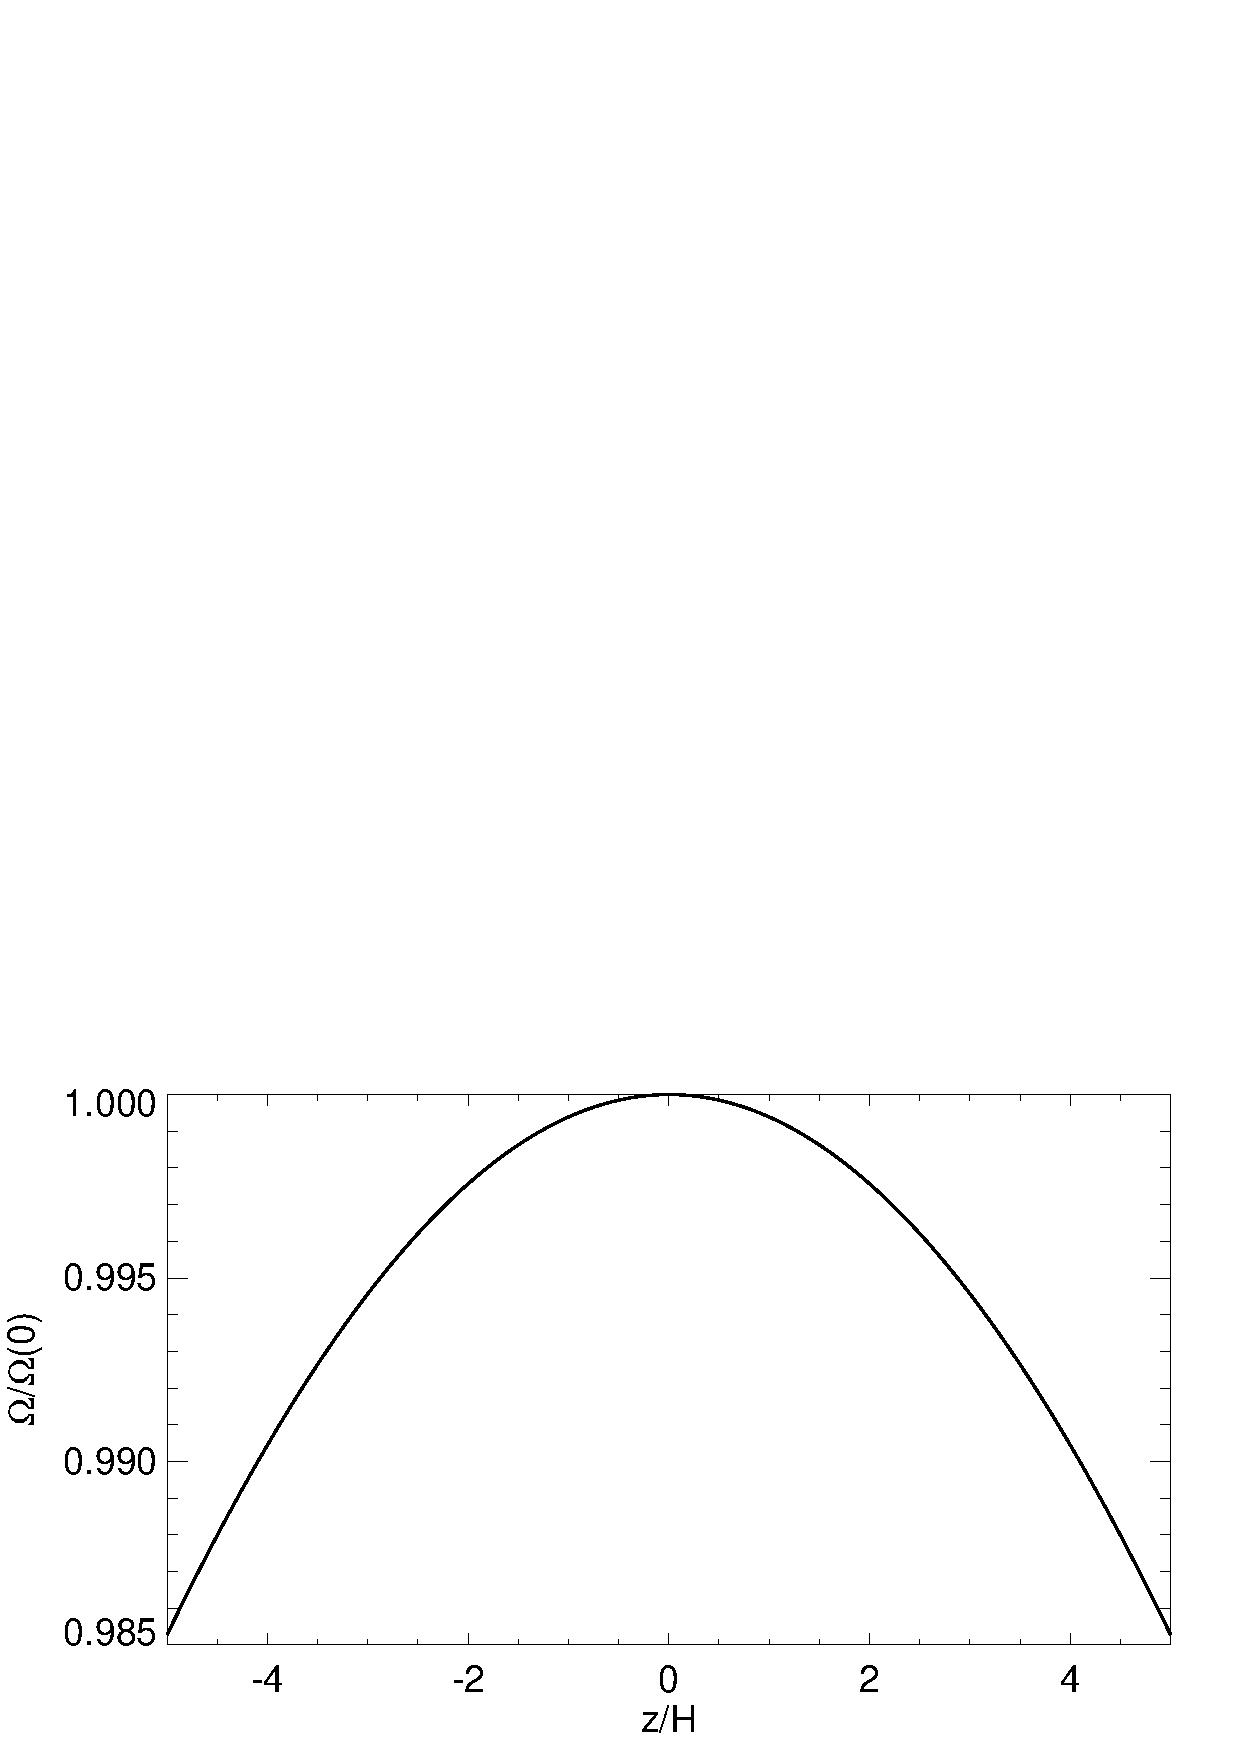
\includegraphics[width=\linewidth,clip=true,trim=0cm 0cm 0cm
  0cm]{figures/omega2} 
  \caption{Equilibrium rotation profile $\Omega(z)$,
    normalized by its mid-plane value, for a disk with $\Gamma=1.011$
    and $(p,q,\epsilon)=(-1.5,-1,0.1)$. 
    \label{omega_z} 
  }
\end{figure}


%behaviour as func of kx 

Fig. \ref{iso_eigen_kx} compares the numerically-obtained eigenvalues
for the fundamental mode and that calculated from
Eq. \ref{simple_growth} (with $L=1$). There is good agreement for  
$\khat\gtrsim10$. The match worsens for decreasing $\khat$ due to the
neglect of global radial structure in the analysis. 

% the low-frequency approximation used to obtain Eq. \ref{sig2_iso} 
% is no longer valid, as $|\omega|$ is not small compared to $\Omega_k$
% for $\khat\lesssim 10$.  

 With rapid thermal relaxation, growth rates are expected to diminish for both $\khat\to 0$
 and $\khat\to \infty$. This is because for $\khat\ll 1$ the radial
  wavelenth is large, but such disturbances are 
  stabilized by by epicyclic motions ($|\omega|\sim
  \kappa$). Disturbances with $\khat\gg 1$ are radially localized, but  
  there is no energy change when fluid elements are perturbed at fixed
  cylindrical radius whilst conserving its angular momentum (since we
  consider axisymmetric perturbations).  


\begin{figure}
  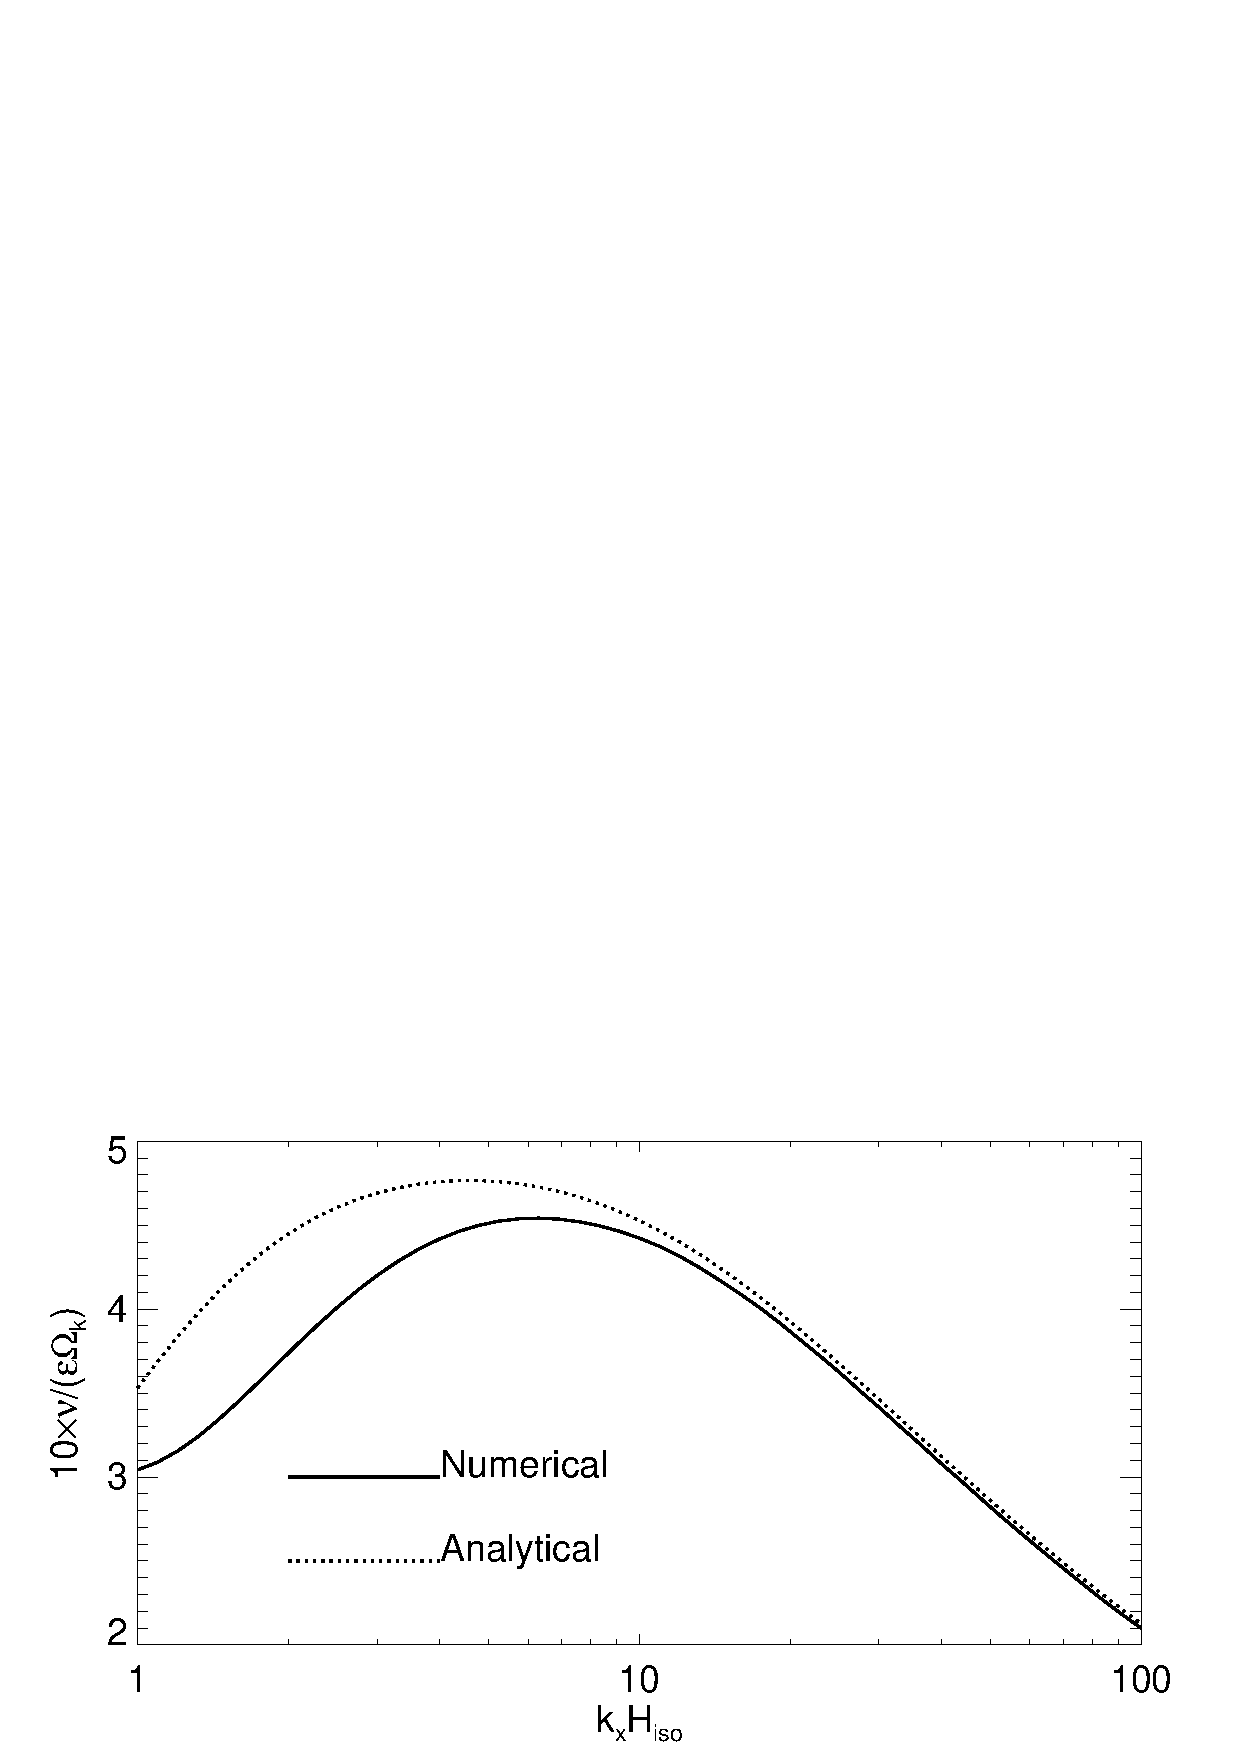
\includegraphics[width=\linewidth,clip=true,trim=0cm 1.75cm 0cm
  0cm]{figures/compare_eigen_imag_iso} 
  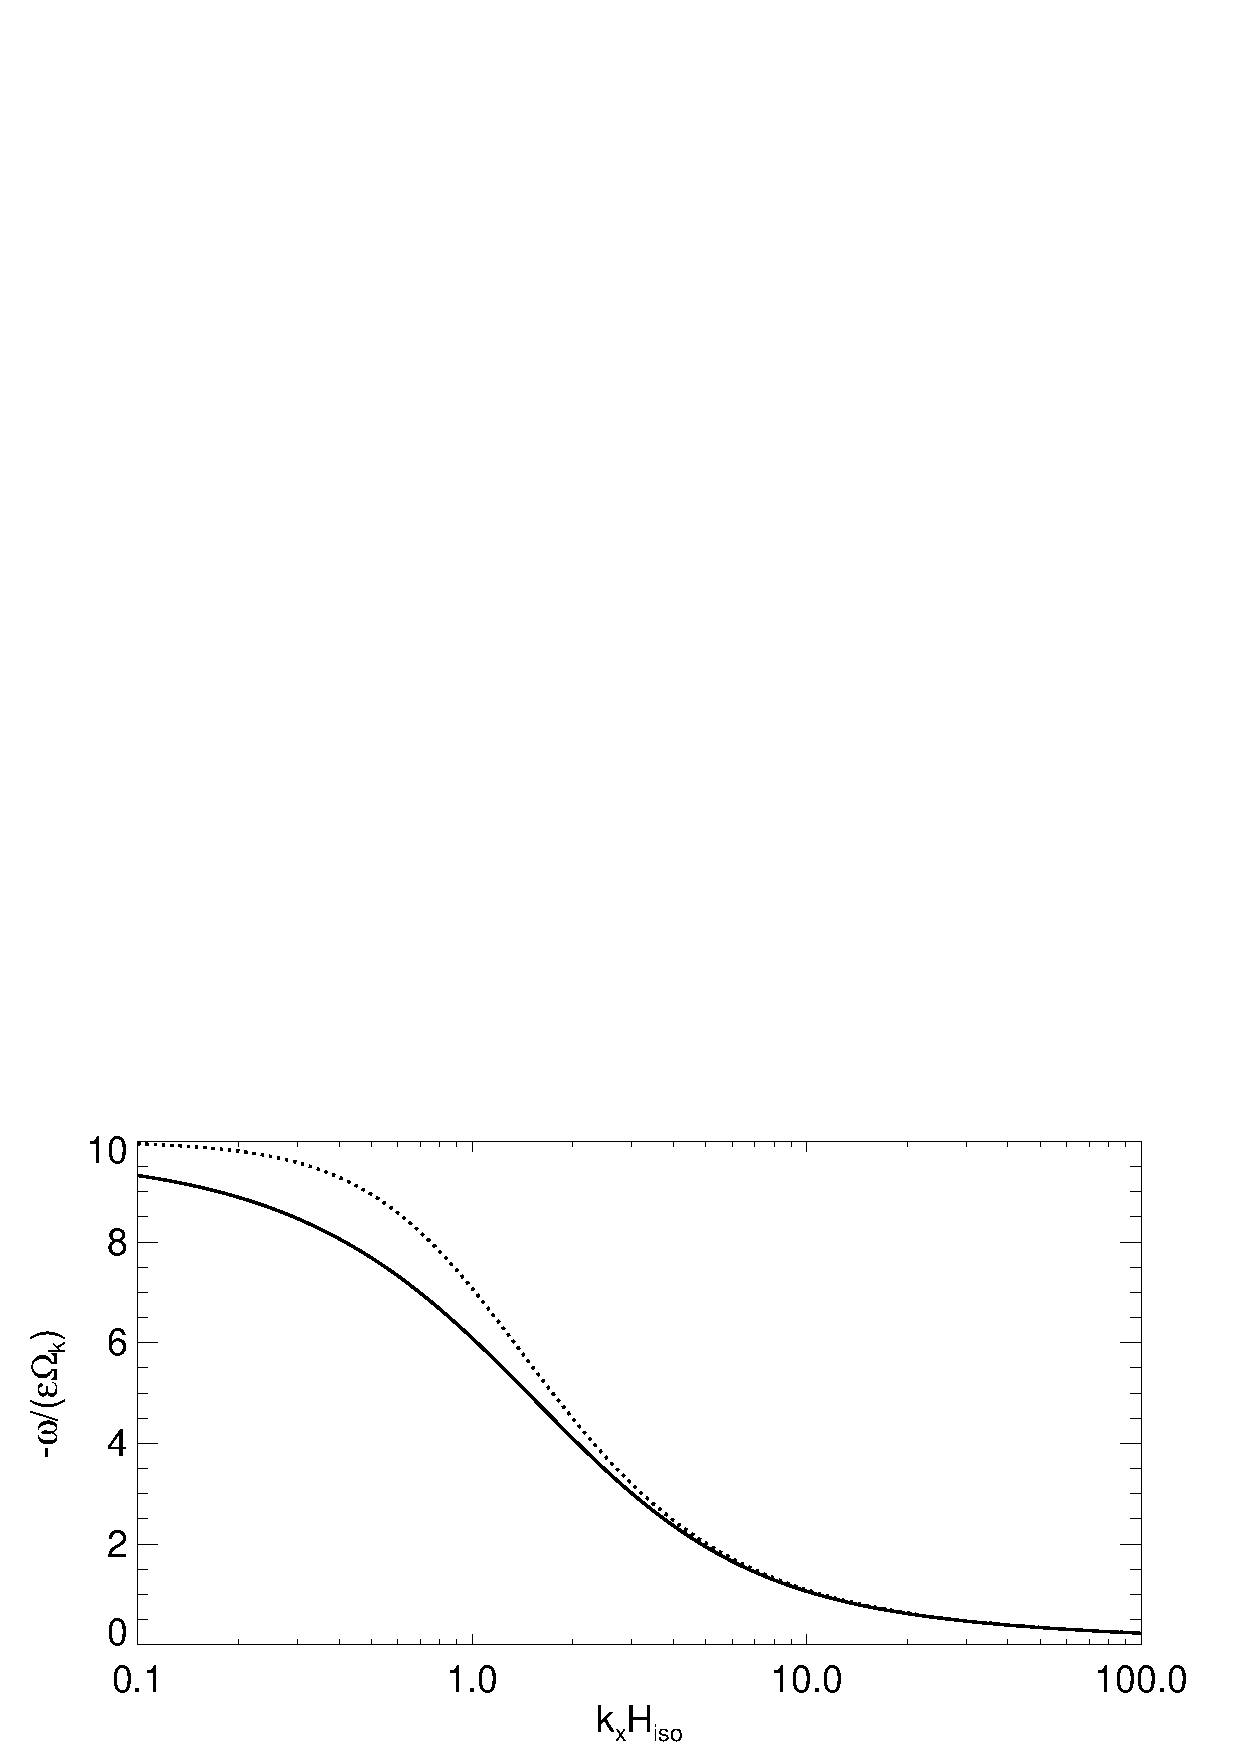
\includegraphics[width=\linewidth,clip=true,trim=0cm 0cm 0cm
  1cm]{figures/compare_eigen_real_iso}
  \caption{Growth rate (top) and real frequency (bottom) of the
    fundamental VSI mode in a disk with $\gamma=\Gamma=1.011$,
    $(p,q,\epsilon)=(-1.5,-1,0.1)$ and
    $\beta=10^{-3}$. The solid (dotted) line is obtained numerically
    (analytically).  
    \label{iso_eigen_kx} 
  }
\end{figure}

Fig. \ref{lowfreq_eigenfunc} compares the fundamental VSI eigenfunction
$W$ for $\khat=1$ and $\khat=20\pi$. The latter value, corresponding
to $k_x= 200\pi/r$, was used by \cite{mcnally14}. We find $W$ is
similar for all $\khat\gtrsim10$ and is proportional to $z$, as
expected for the fundamental mode according to explicit solutions
developed in Appendix \ref{iso_explicit}. For completeness we show the
corresponding eigenfunctions in vertical velocity in
Fig. \ref{lowfreq_eigenfuncvz}. The fundamental mode
consists of zero nodes in $\delta v_z$. 

%For $\khat\lesssim 10$, e.g. $\khat=1$ in 
%Fig. \ref{lowfreq_eigenfunc}, the perturbation magnitude near the
%boundaries begin to dominate. For even smaller $\khat\lesssim 1$ (not
%shown) we find the perturbation is almost entirely concentrated at the
%boundaries. However, our radially-local approximation is not valid for 
%such small wavenumber perturbations. 

\begin{figure}
  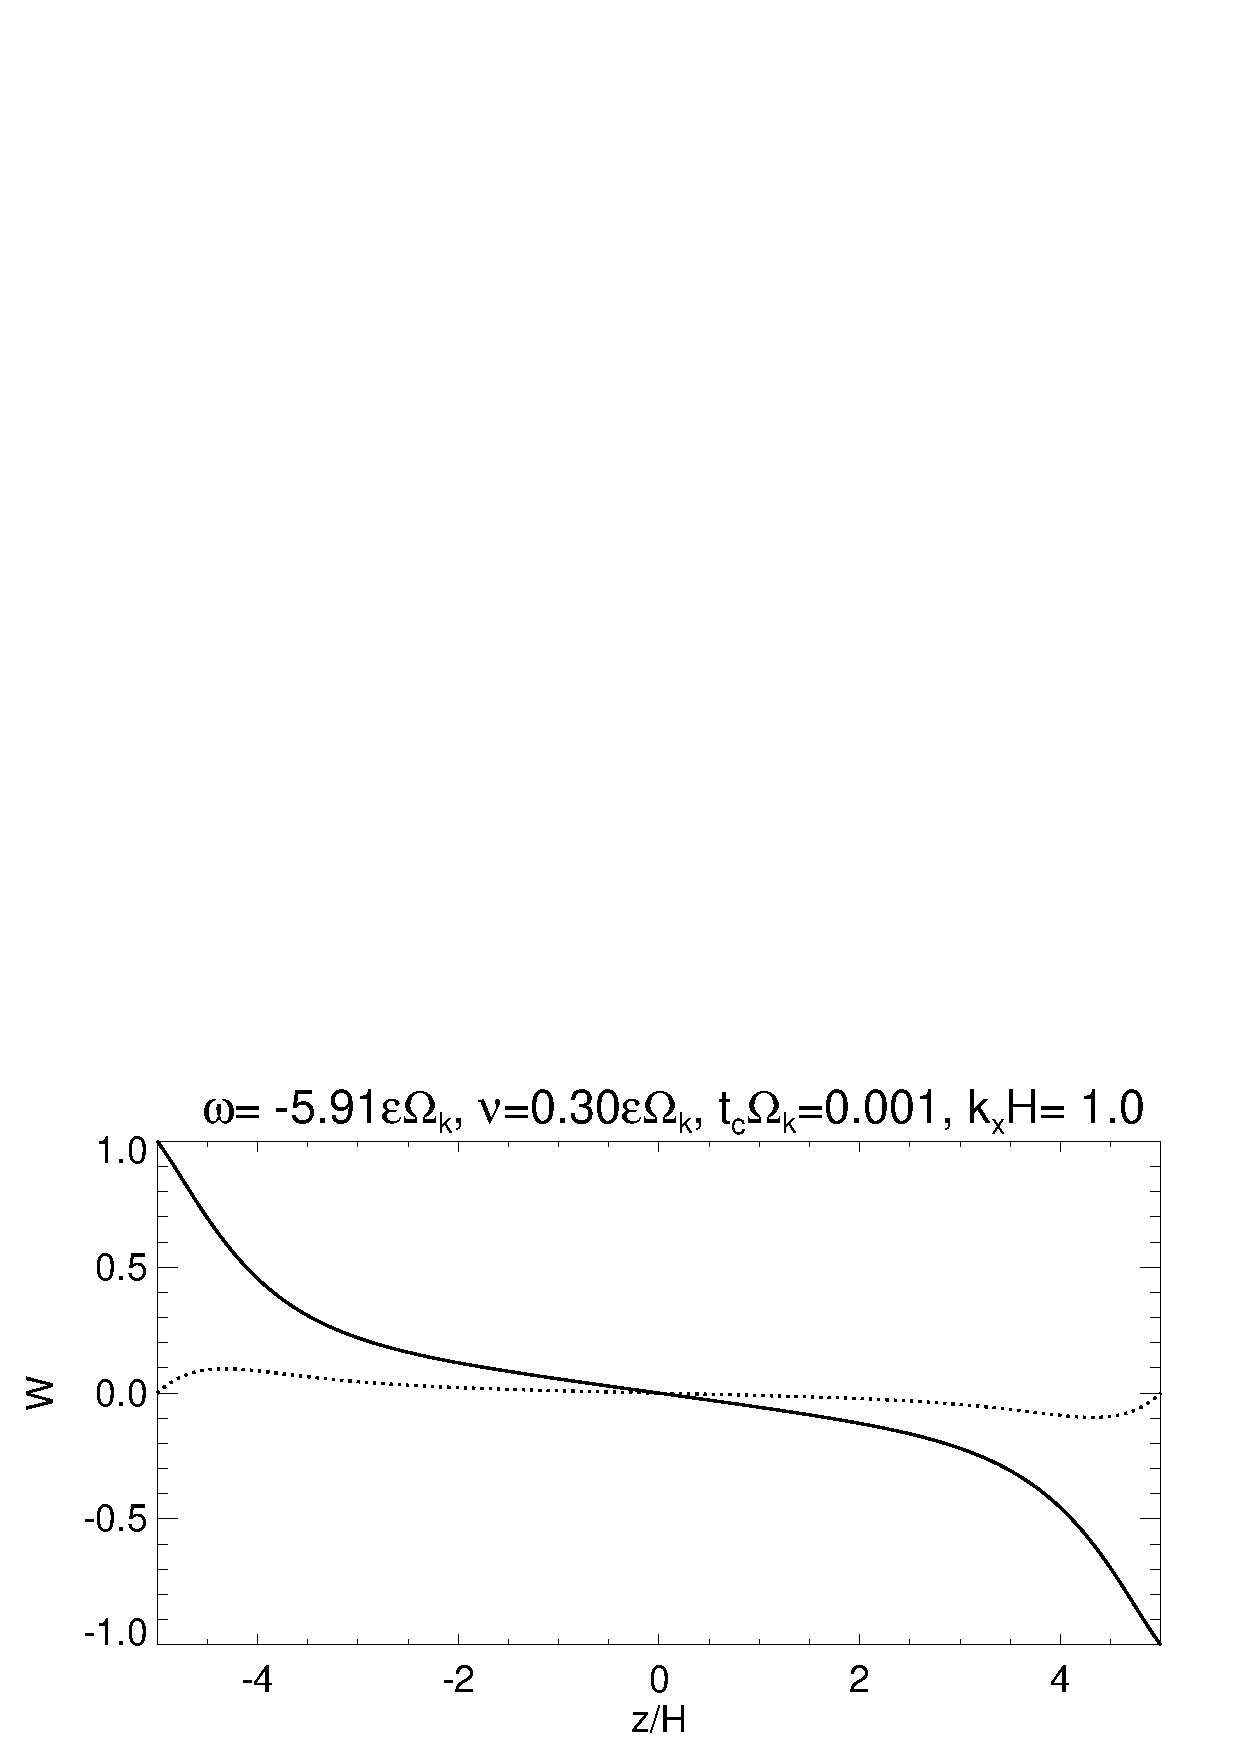
\includegraphics[width=\linewidth,clip=true,trim=0cm 1.75cm 0cm
  0cm]{figures/eigenvector_iso_kx1} 
  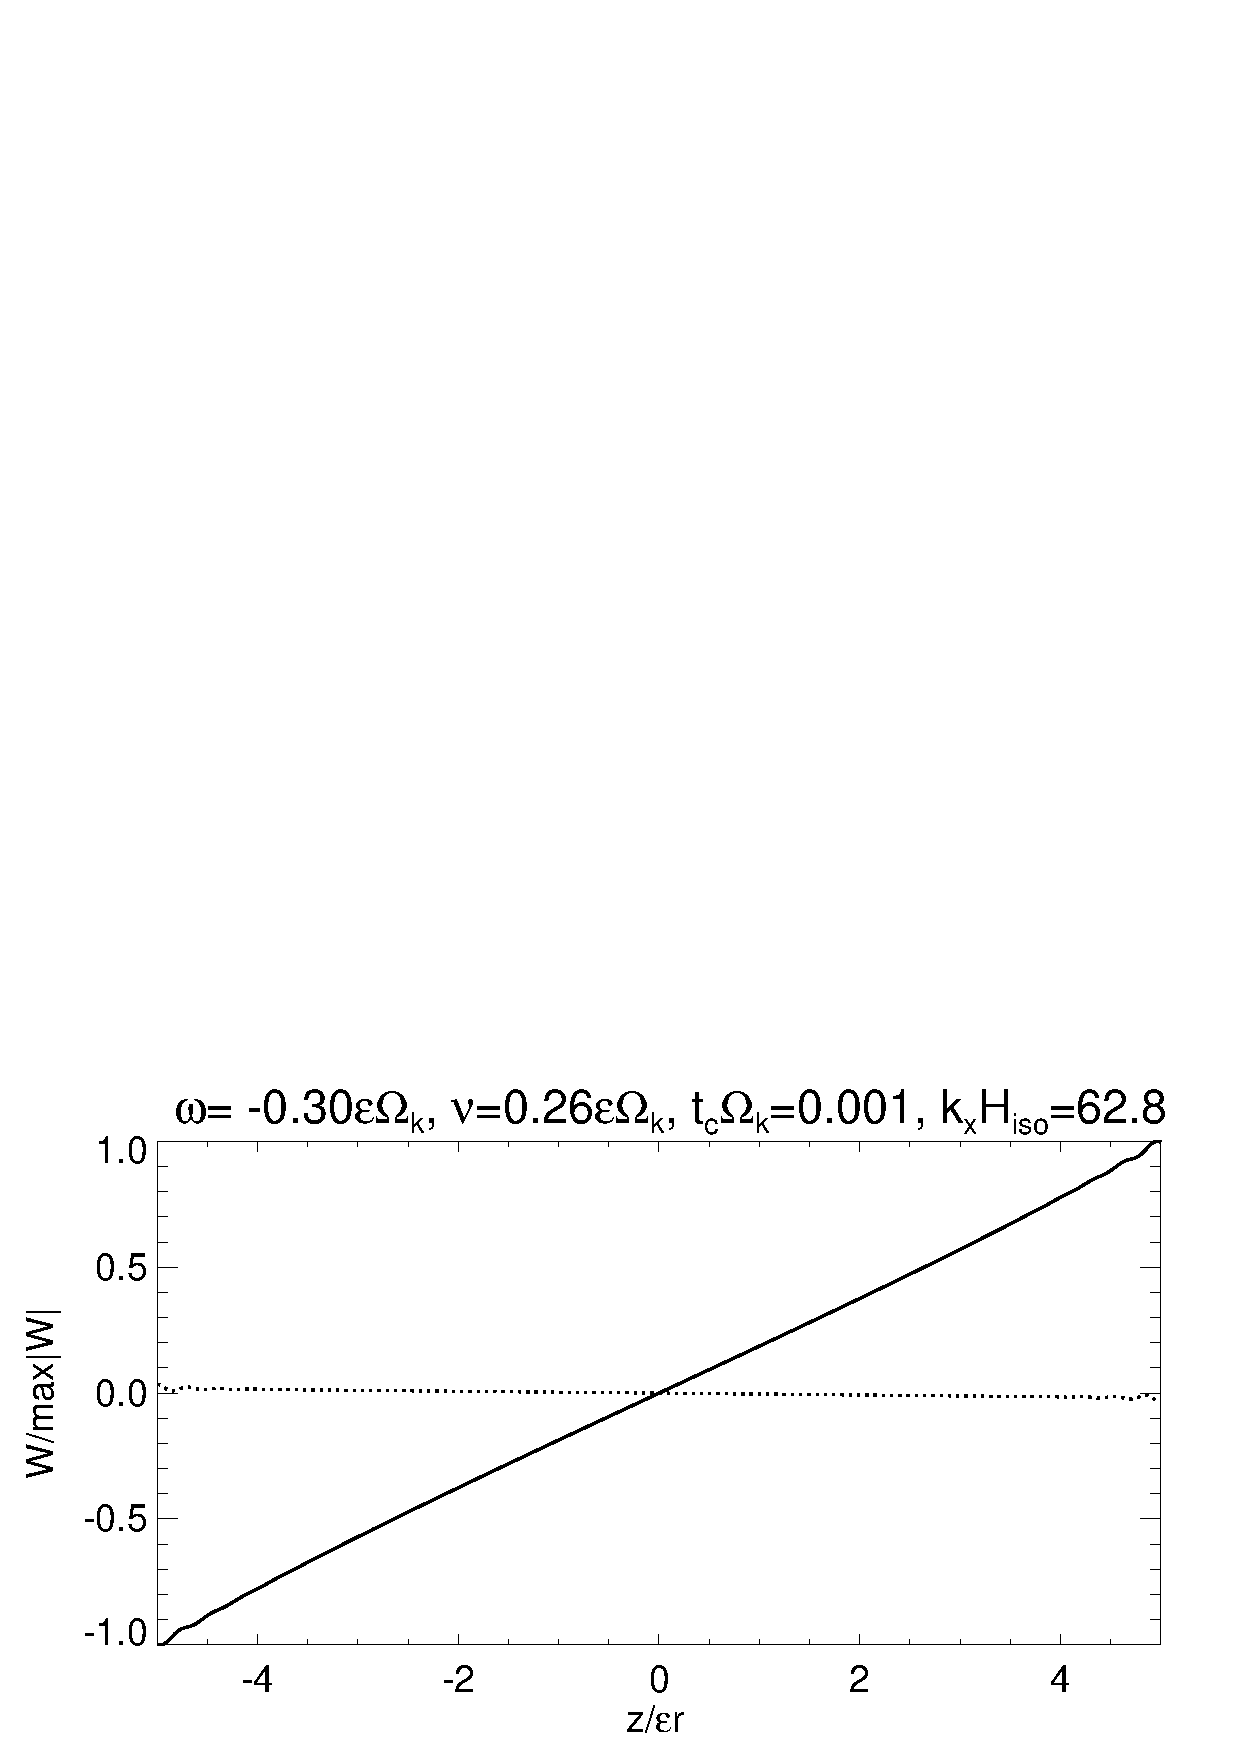
\includegraphics[width=\linewidth]{figures/eigenvector_iso_kx60}
  \caption{Eigenfunction $W$ of the fundamental VSI for perturbation
    wavenumber $\khat=1$ (top) and $\khat=20\pi$ (bottom). The real 
    (imaginary) parts of $W$ are plotted as solid (dotted) lines. % The
    % eigenfunction has been normalized such that $\imag(W)=0$ at the
    % vertical boundaries and $\mathrm{max}|W|=1$. 
    \label{lowfreq_eigenfunc}
  }
\end{figure}

\begin{figure}
  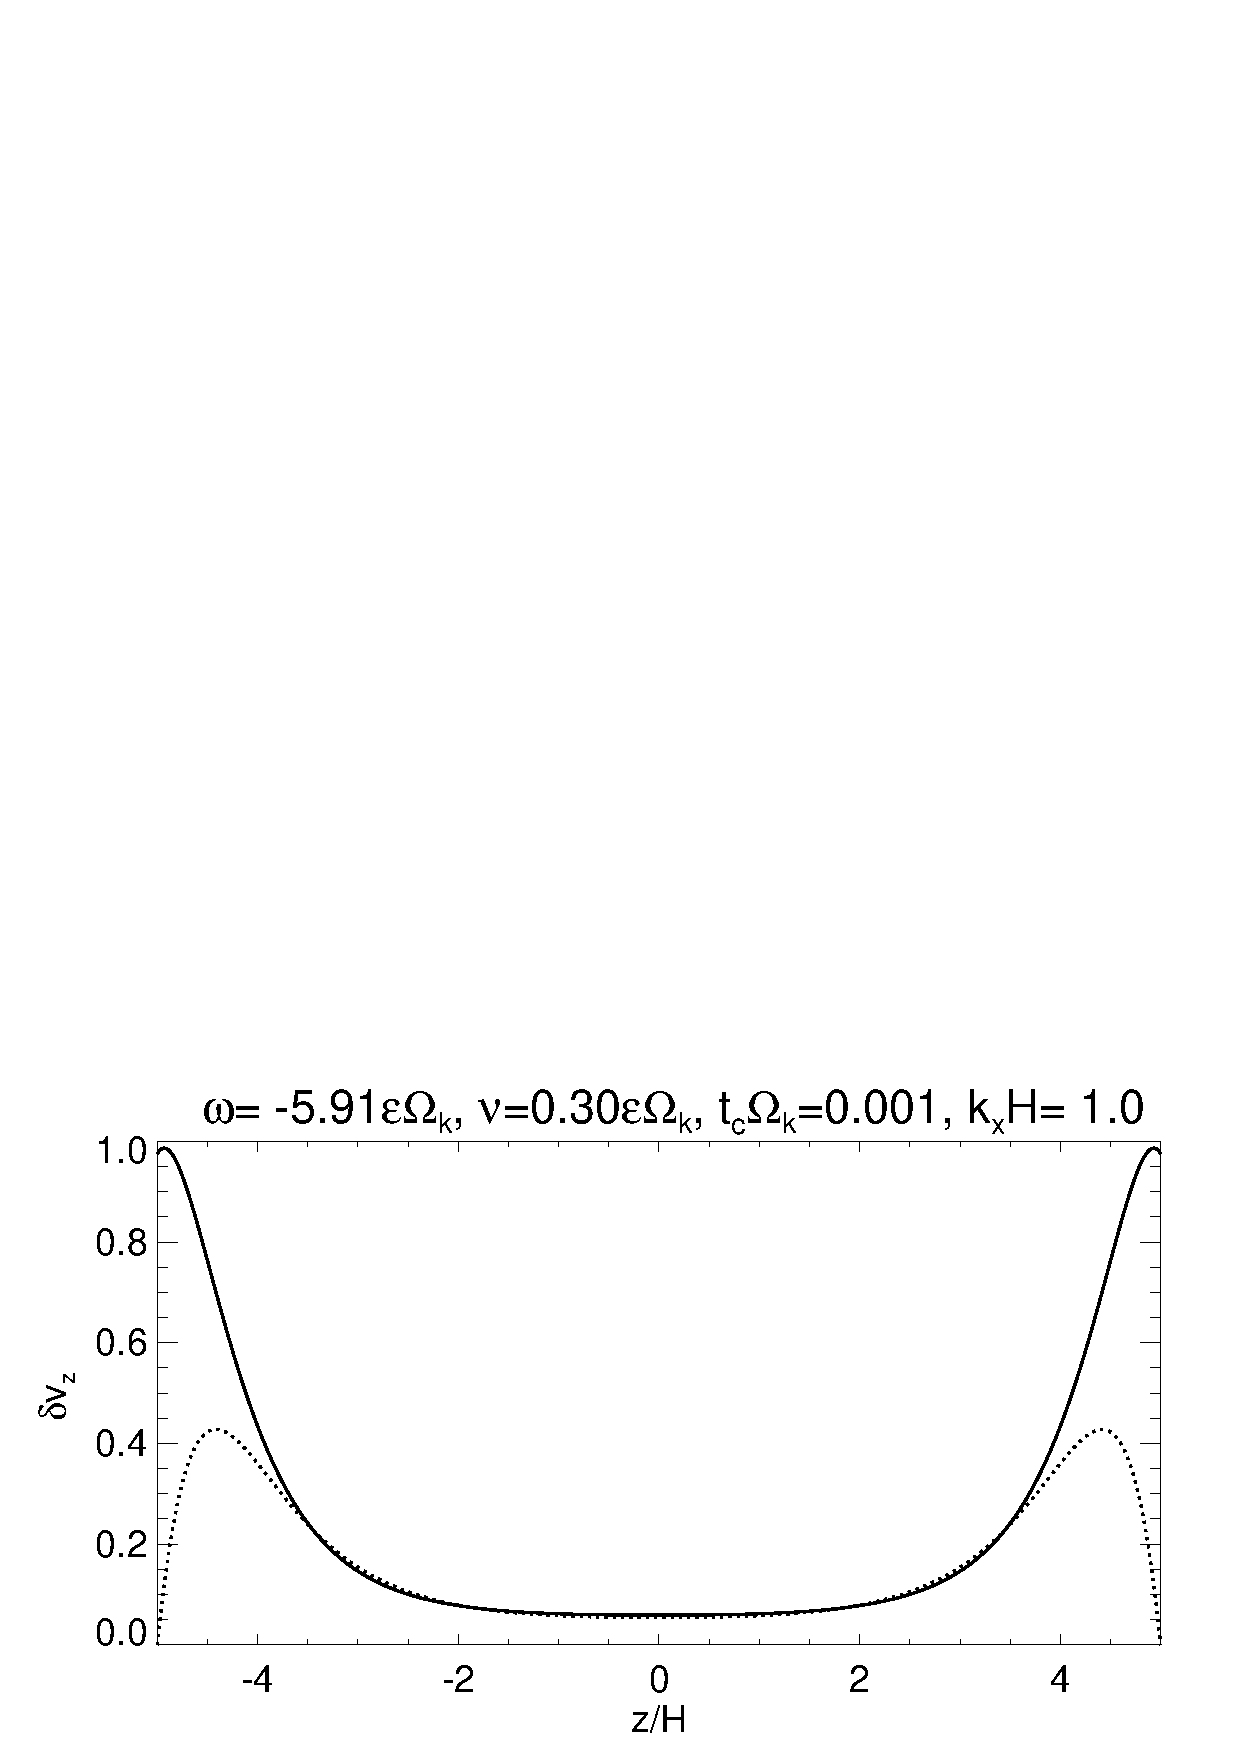
\includegraphics[width=\linewidth,clip=true,trim=0cm 1.75cm 0cm
  0cm]{figures/eigenvectorvz_iso_kx1} 
  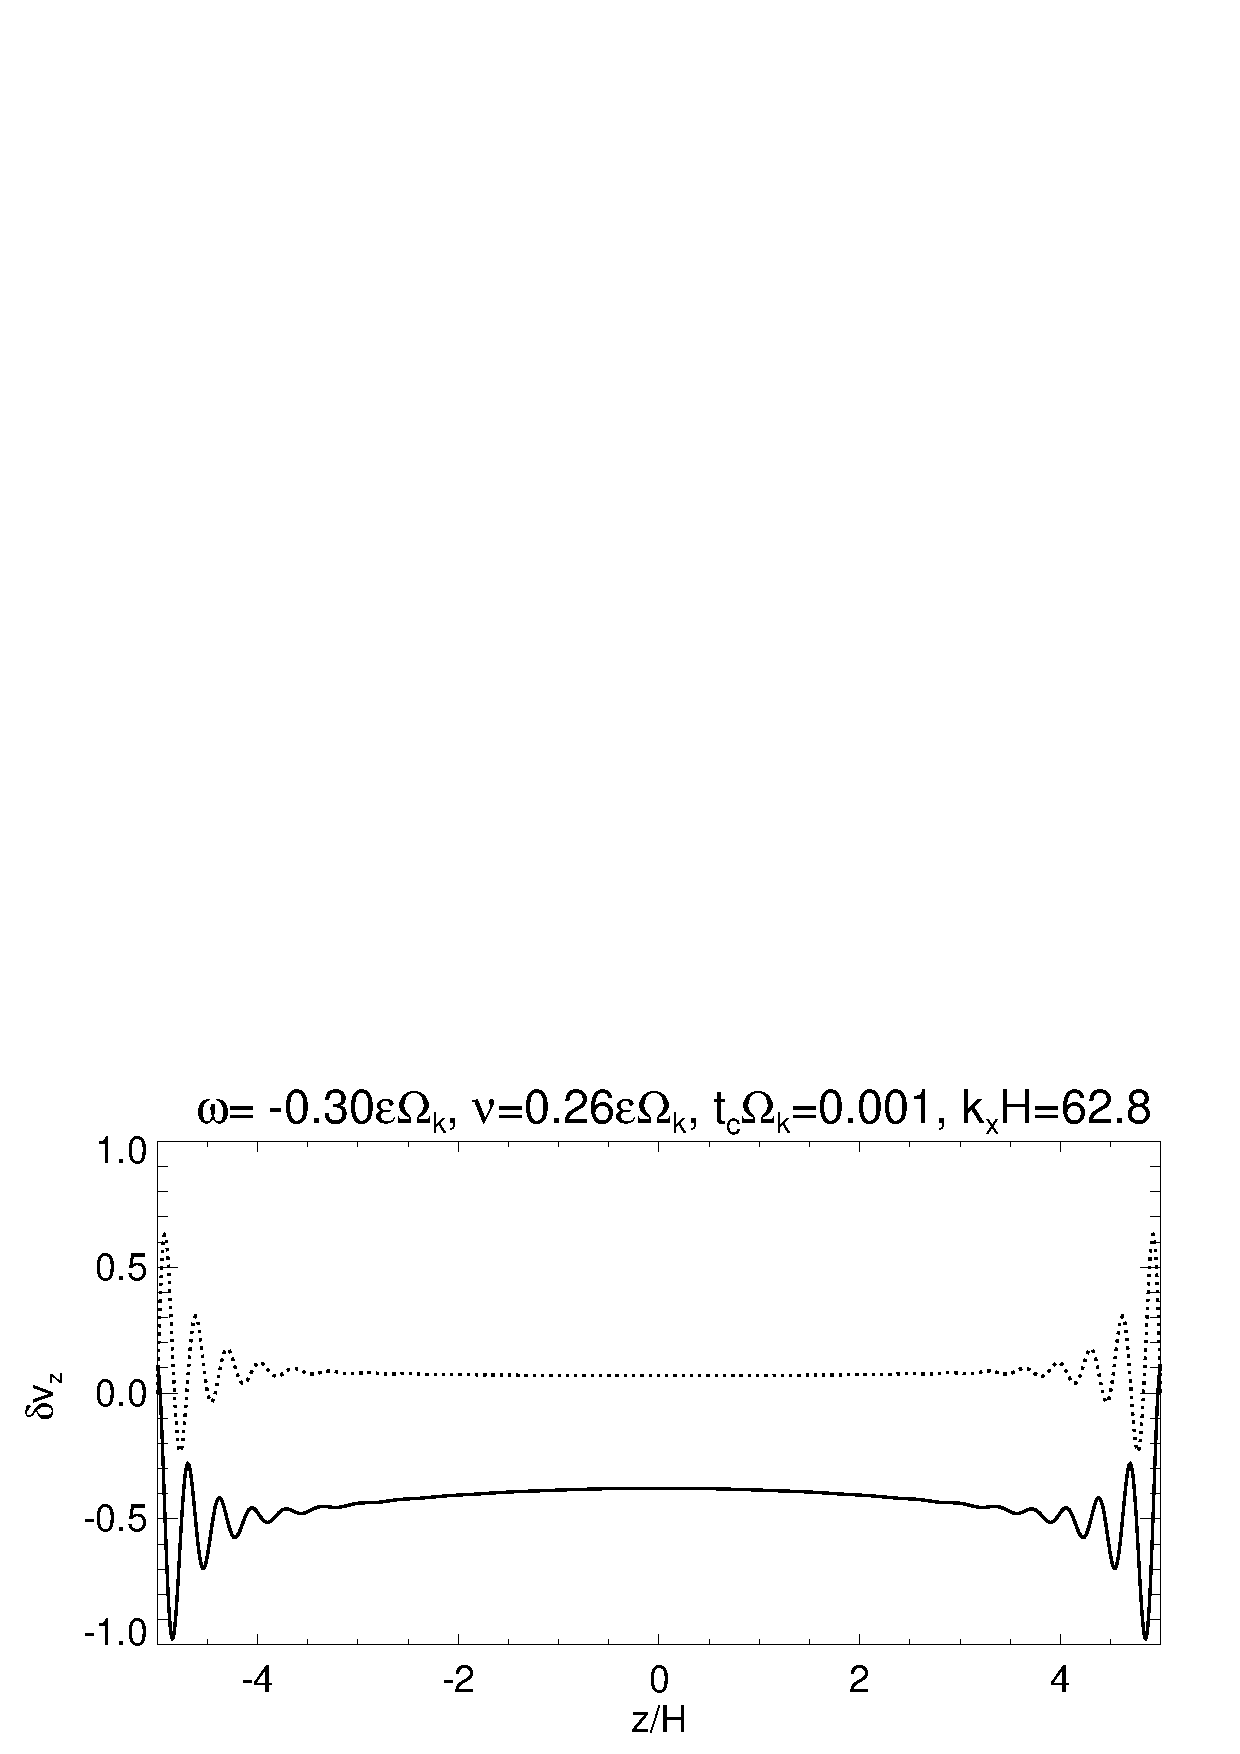
\includegraphics[width=\linewidth]{figures/eigenvectorvz_iso_kx60}
  \caption{Same as Fig. \ref{lowfreq_eigenfunc} but for the vertical
    velocity eigenfunctions.
    \label{lowfreq_eigenfuncvz}
  }
\end{figure}

In Fig. \ref{lowfreq_eigen} we plot the eigenvalues 
$\sigma = \omega + \ii\nu$ found for $\khat=20\pi$. This plot is
similar to Fig. 3 in \cite{mcnally14}. The fundamental mode has the
smallest $|\sigma|$, for which the eigenvalue calculated from
Eq. \ref{simple_growth2} with $L=1$ and the numerically-obtained value are   
\begin{align*}
  (\omega,\nu) = (-0.3053,0.2605)\epsilon\Omega_k &\quad \text{(from
    Eq. \ref{simple_growth2})},\\
  (\omega,\nu) = (-0.3010,0.2575) \epsilon \Omega_k &\quad \text{(numerical)}.
\end{align*}
This agreement is surprisingly good given the number of approximations
used to obtain Eq. \ref{simple_growth2}, which also imposes a different
boundary condition to that in the numerical calculation. These values
are also close to that found by \cite{mcnally14}. The eigenfrequency
is not sensitive to the vertical boundary condition because the
expression for $\sigma$, given by Eq. \ref{integral_relation1},
involve integrals with $\rho$ as the   weight function, which rapidly
decays away from the midplane. 

\begin{figure}
  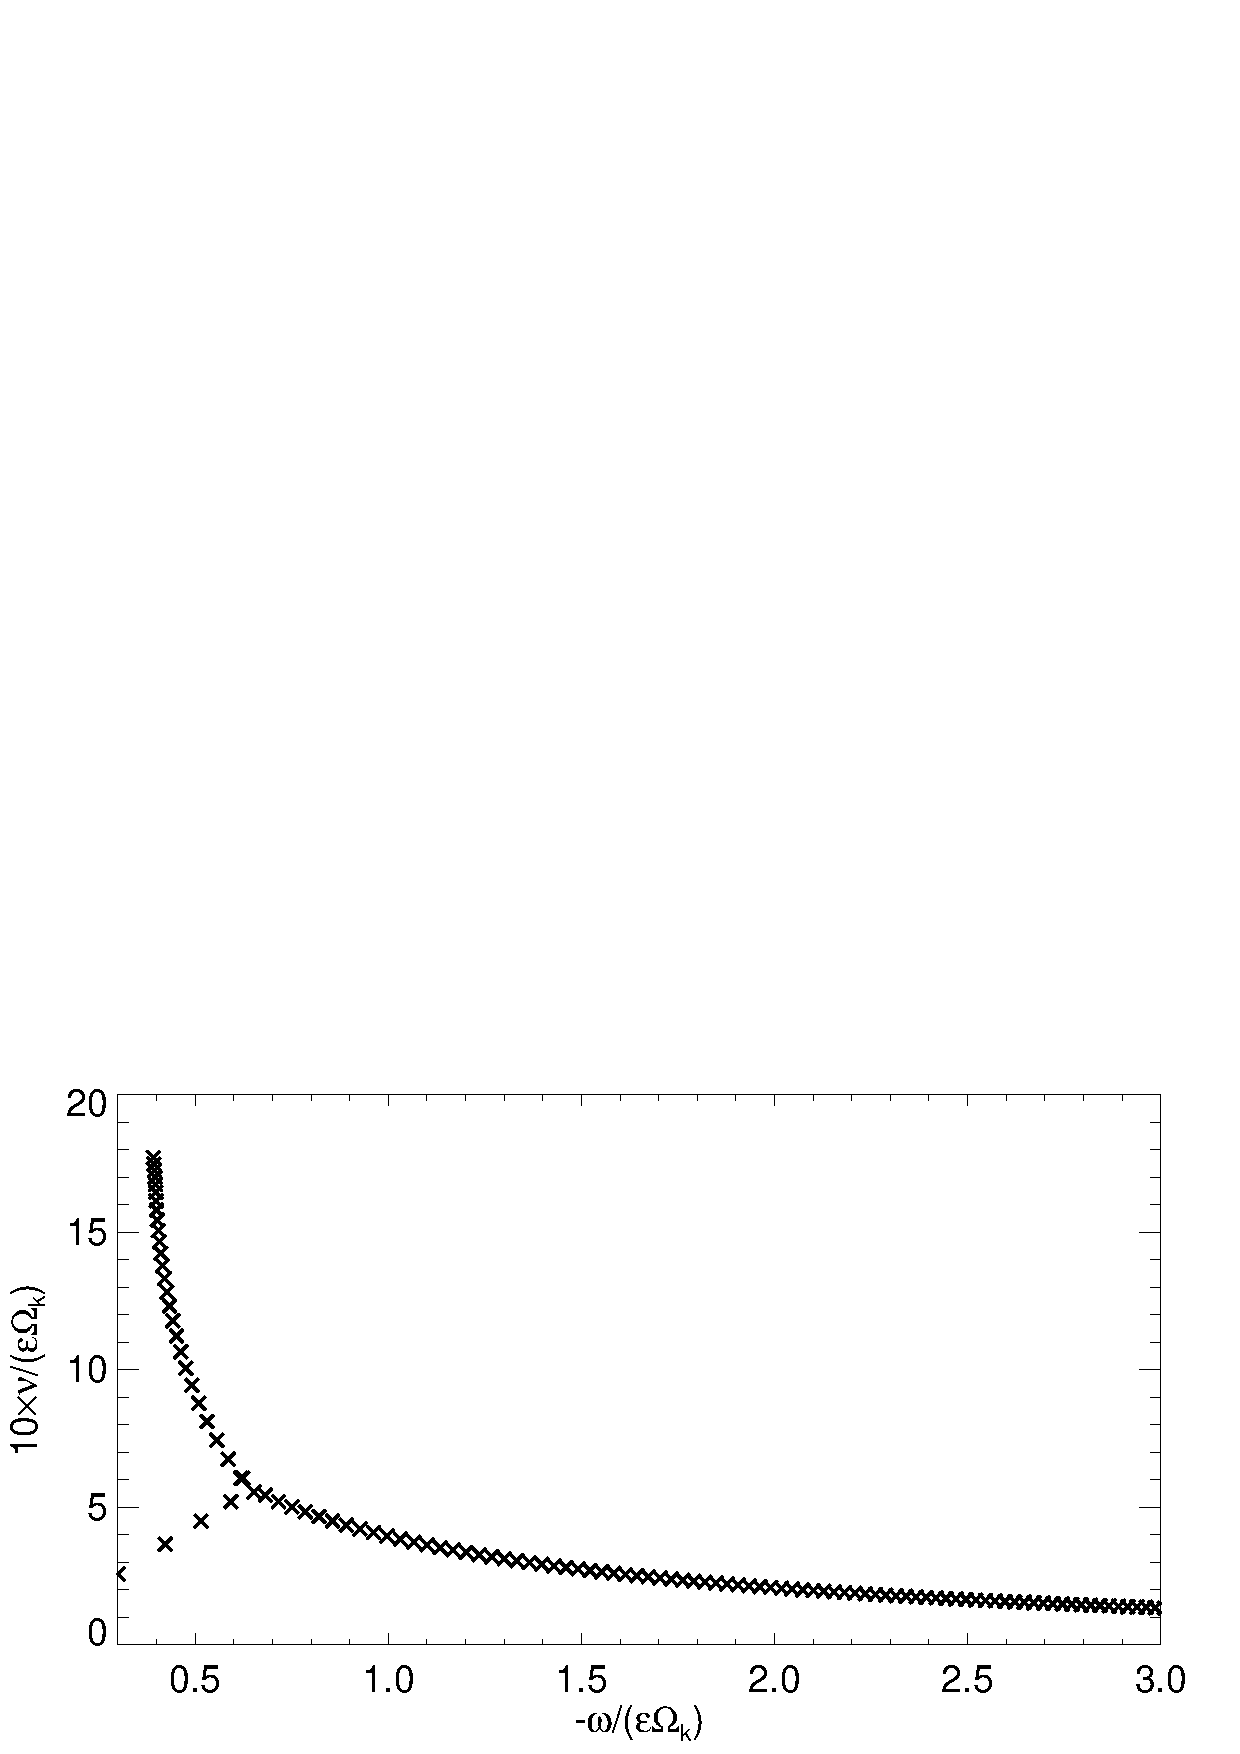
\includegraphics[width=\linewidth]{figures/eigenvalues_iso}
  \caption{Eigenvalues of perturbations with wavenumber $\khat=20\pi$
    in a neutrally-stratified, nearly-vertically isothermal disk
    ($\gamma=\Gamma=1.011$) with $(p,q,\epsilon)=(-1.5,-1,0.1)$ and
    $\beta=10^{-3}$. \label{lowfreq_eigen} 
  }
\end{figure}

\subsection{Effect of thermal relaxation}
We now consider stably stratified disks ($\gamma > \Gamma$) with
thermal relaxation. Here, we use a slightly  
different disk model with $\epsilon=0.05$ and $\gamma=1.4$, as 
adopted in simulations performed by \cite{nelson13}. Other parameters 
are unchanged from the previous section.  

Fig. \ref{bcrit_compare1} shows the growth rate $\nu$ of the
fundamental VSI as a function of $\beta$ for $\khat\in[1,10^2]$. We
also plot the critical thermal relaxation timescale
$\beta_\mathrm{crit}=0.125$ given by Eq. \ref{iso_vsi_cond} for the present
disk parameters.

For $5\lesssim\khat\lesssim30$, we find $\beta_\mathrm{crit}$ provides an
accurate prediction of the upper limit to the thermal relaxation 
timescale for  the fundamental mode. For smaller $\khat$,
$\beta<\beta_\mathrm{crit}$ is a sufficient condition for
instability. For larger $\khat$, we find $\nu$ does not reach zero but
rapidly decreases as $\beta$ approaches and increases beyond
$\beta_\mathrm{crit}$. In the latter case we find the perturbation
acquires large amplitudes near the vertical boundaries. Boundary
conditions may thus may play a role for these modes that is not
accounted by our analytical discussion.  

Fig. \ref{bcrit_compare1} shows that 
$\beta_\mathrm{crit}$ is a good indication for the maximum
thermal relaxation timescale to permit the fundamental VSI. For
$\beta\lesssim O(10^{-2})$, growth rates are insensitive to thermal
relaxation. For this disk model, \citeauthor{nelson13}
found a thermal relaxation timescale of $\beta\gtrsim 0.6$ stabilized
the VSI in non-linear hydrodynamic simulations. This is consistent
with our results.   

It is interesting to note that there is a thermal relaxation timescale that
maximizes the mode decay rate for $1\lesssim \khat \lesssim 30$. Here,
it is $\beta\simeq1$---$2$ or about $0.1$---$0.3$ orbital
periods. This is in fact consistent with Fig. 12 of \cite{nelson13}
where the perturbed kinetic energy in their numerical simulations was
observed to decay most rapidly for a thermal timescale of $\sim 0.1$
orbits.     

%implications for nonlinear sims?

 \begin{figure}
   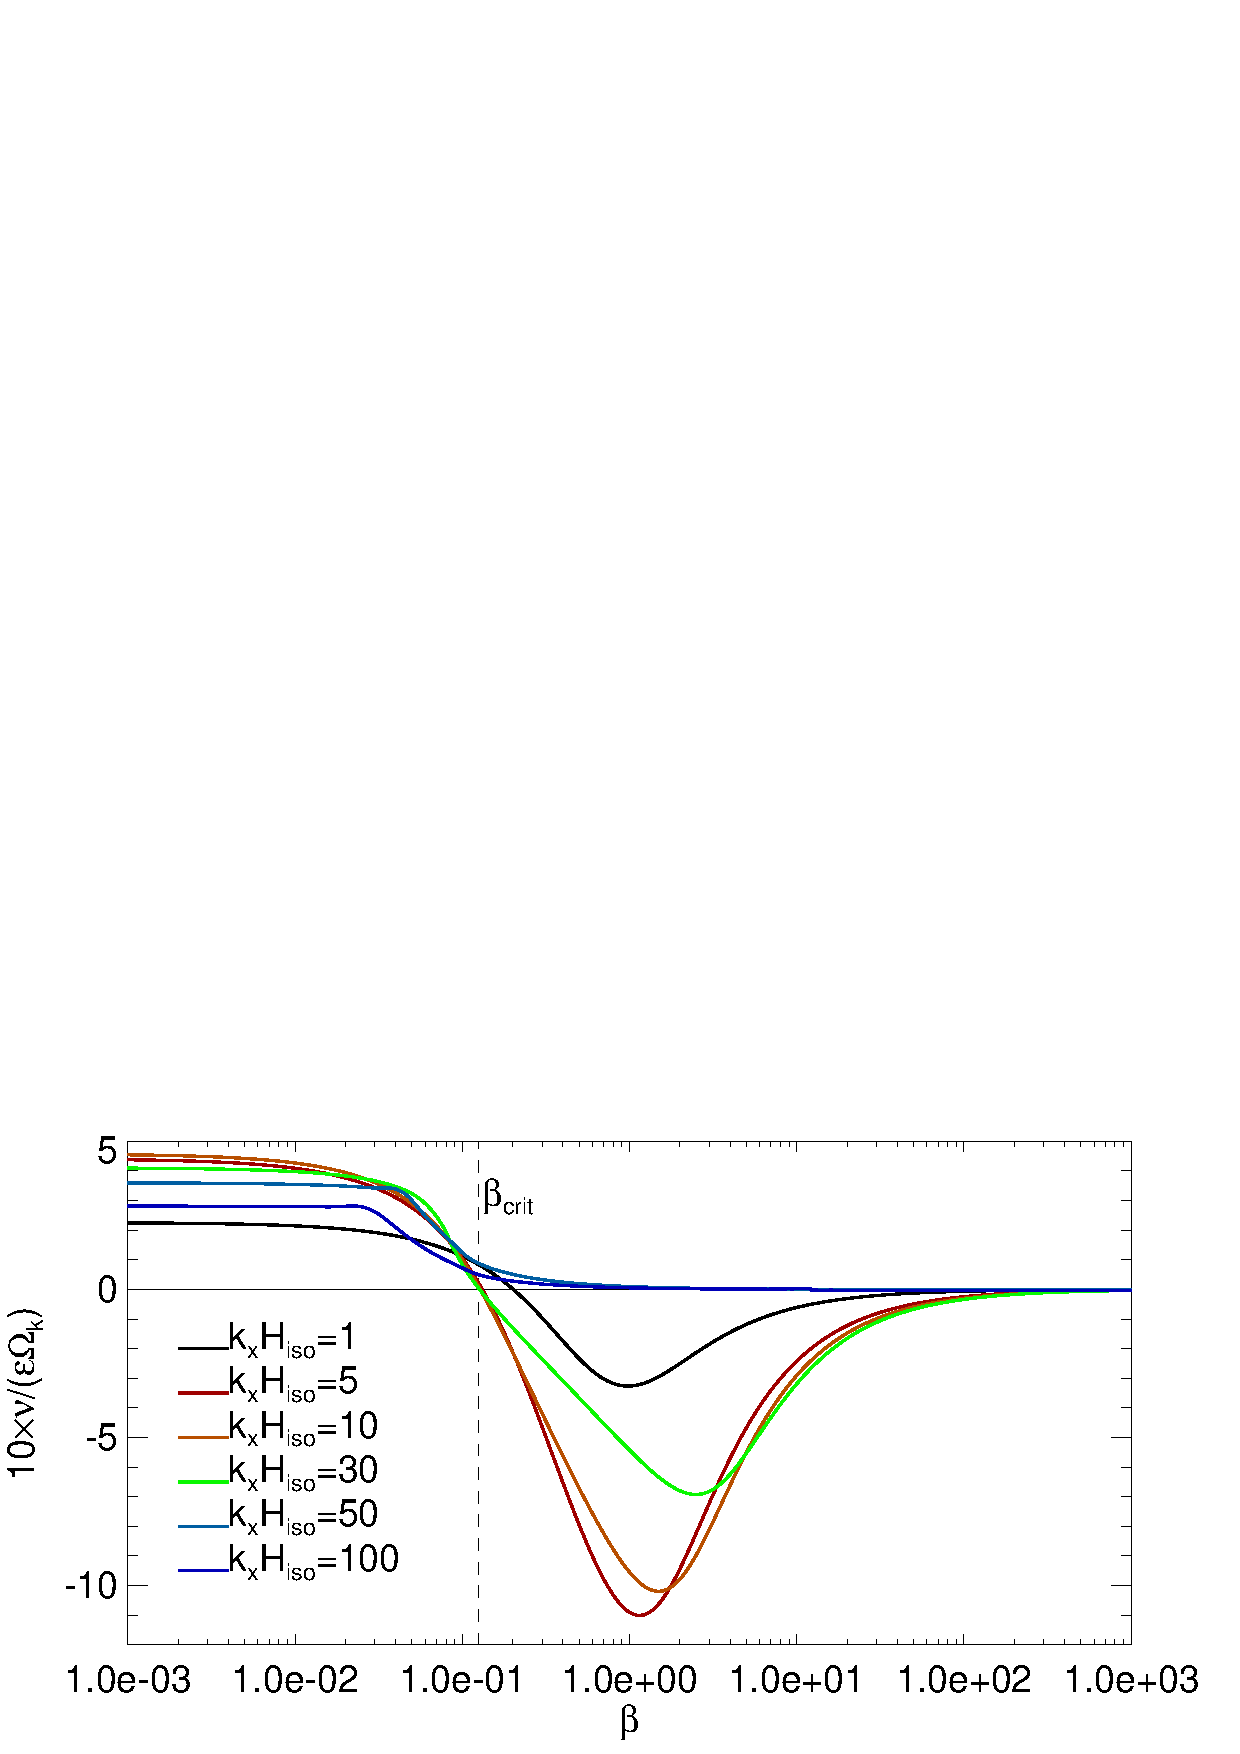
\includegraphics[width=\linewidth]{figures/gcorr_compare2} 
   \caption{Growth rate of the fundamental VSI as
     a function of the thermal relaxation timescale $\beta$. The disk
     parameters are $\Gamma=1.011$, $\gamma=1.4$, and 
     $(p,q,\epsilon)=(-1.5,-1,0.05)$. The vertical line
     is the critical thermal timescale $\beta_\mathrm{crit}$  obtained
     from Eq. \ref{iso_vsi_cond}. 
     \label{bcrit_compare1}}   
 \end{figure} 

% Fig. \ref{relax_growth_num} shows the growth rates of the fundamental  
% mode as a function of $\khat$. This plot is largely consistent with  
% Fig. \ref{relax_disp_fig} except for $\khat\lesssim 1$
% where the low-frequency approximation fails. (In any case, the local model not valid
% for $\khat\ll1$.) For $\khat\gtrsim 10$ introducing thermal
% relaxation rapidly stabilizes the fundamental mode. 


% Fig. \ref{relax_growth_num} also confirms our analytical discussion that
% introducing a small but finite cooling time stabilizes the fundamental
% VSI, but there is a preferable wavenumber that maximizes this effect (\S\ref{relax_pert}).
% This occurs at $\khat= O(10)$ for the current disk model. 

% \begin{figure}
%    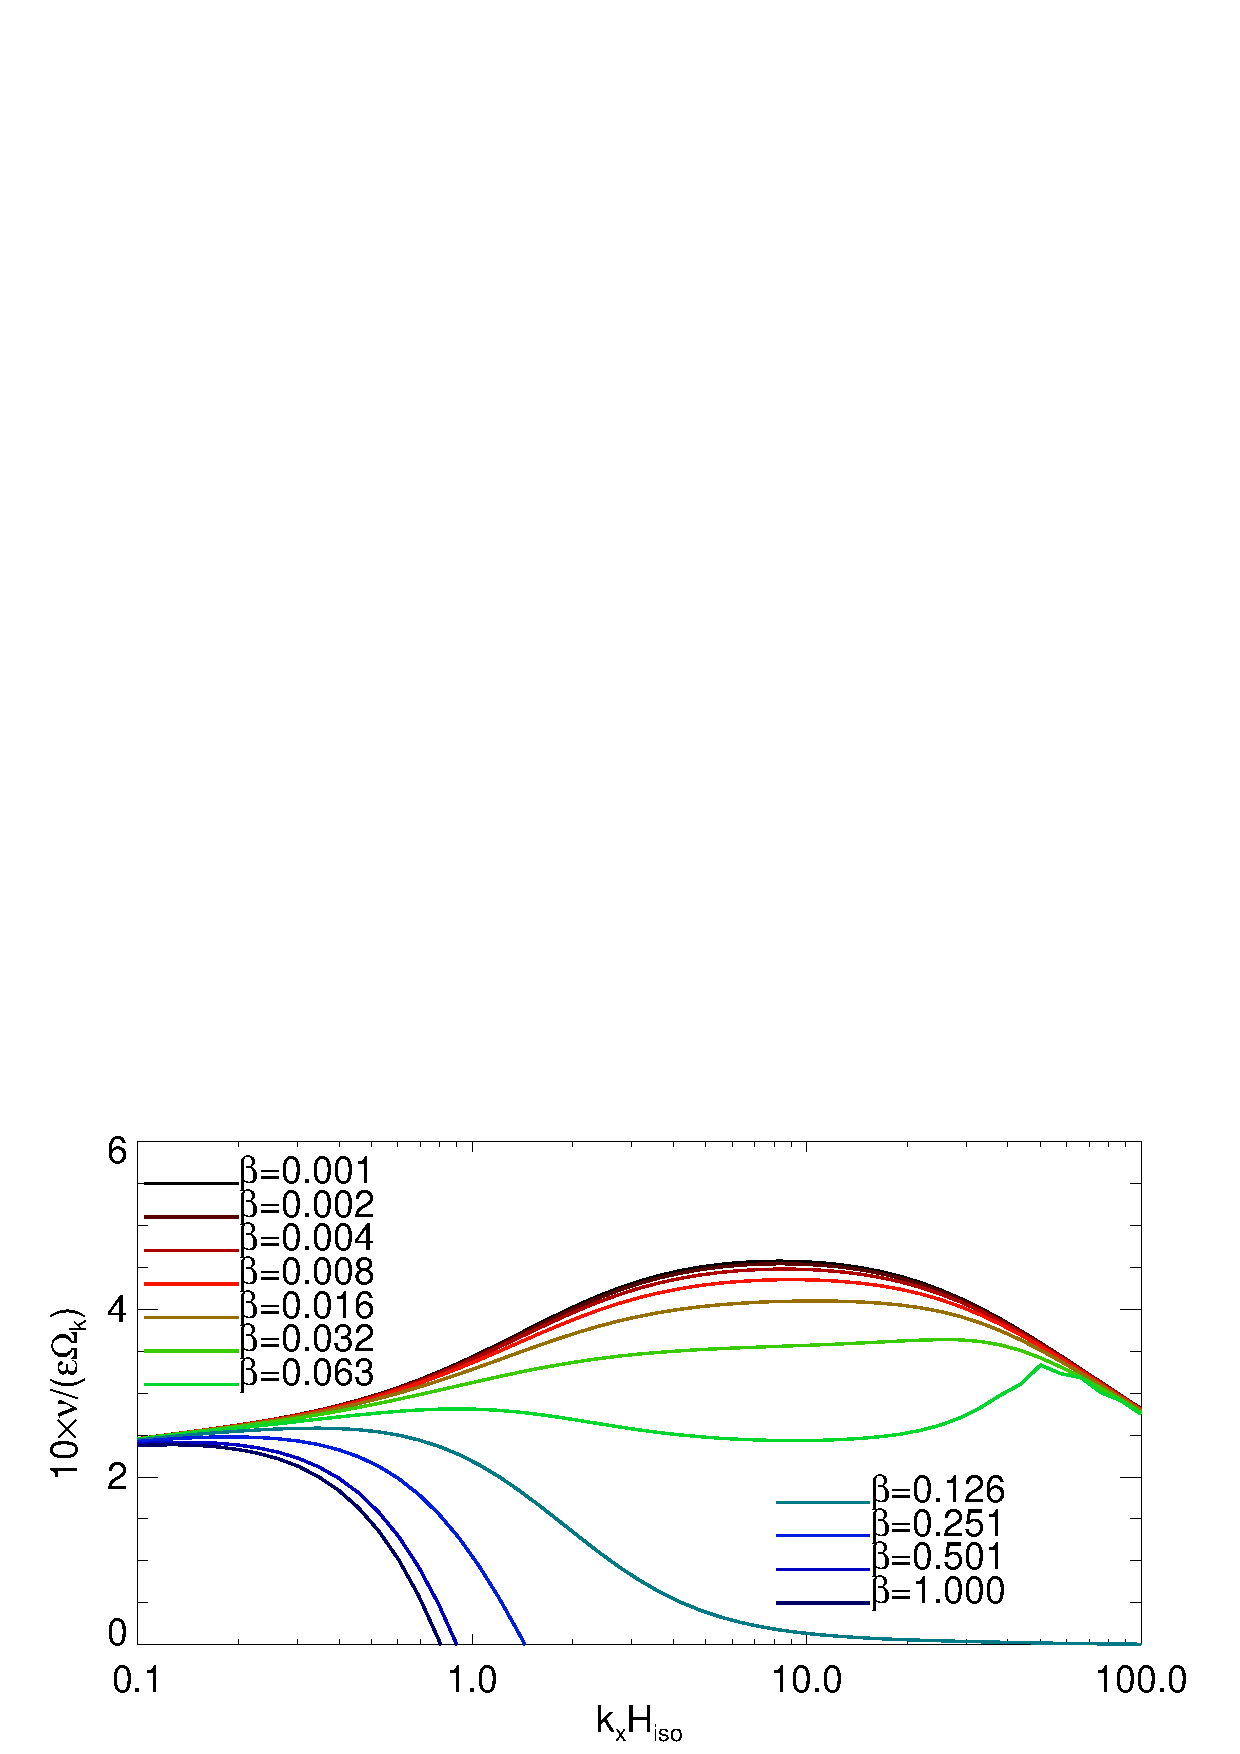
\includegraphics[width=\linewidth,clip=true,trim=0cm 0.0cm 0cm
%    0cm]{figures/compare_eigen_imag_bloop} 
%   % 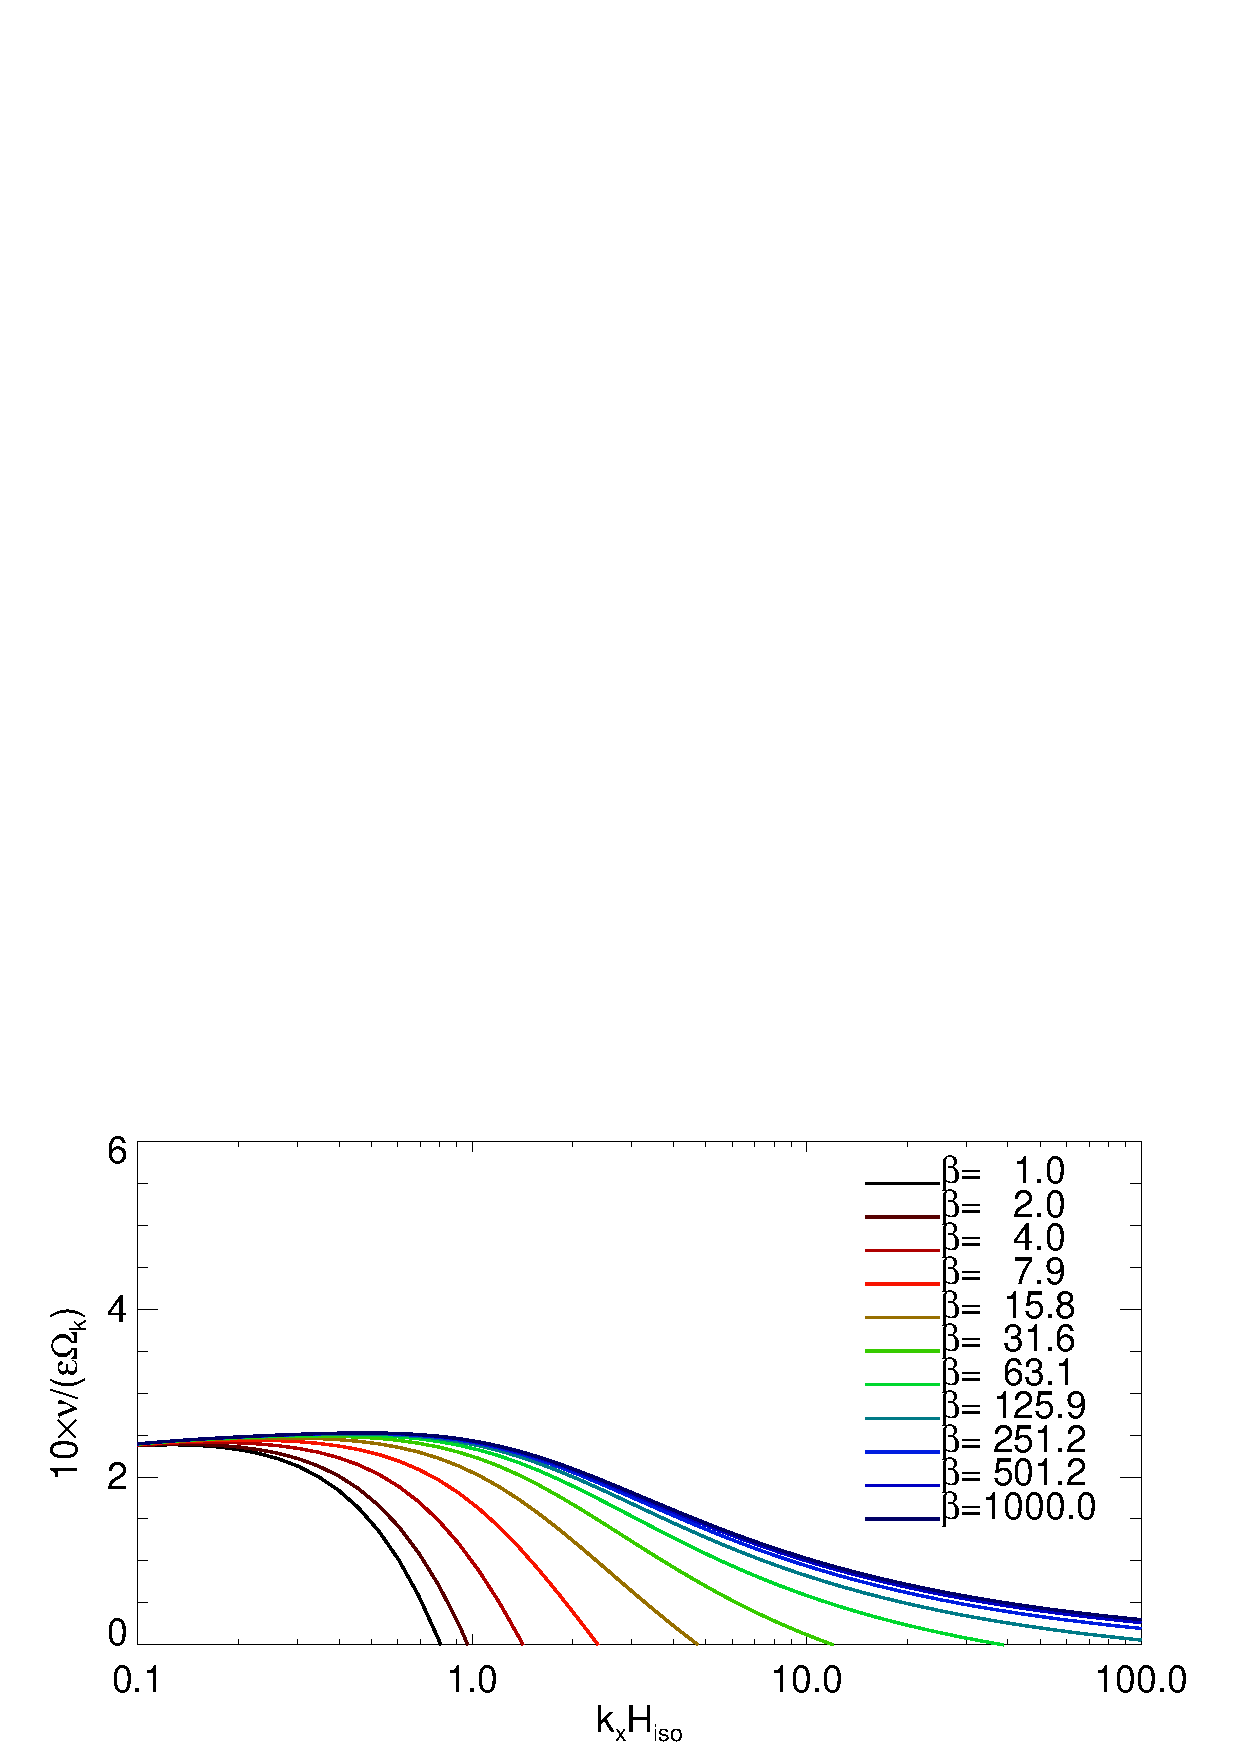
\includegraphics[width=\linewidth,clip=true,trim=0cm 0cm 0cm
%   % 1cm]{figures/compare_eigen_imag_bloop2} 
%   \caption{Growth rates of the fundamental VSI mode in 
%     nearly-vertically isothermal disks ($\Gamma=1.011$) with
%     $(p,q,\epsilon)=(-1.5,-1,0.05)$, evolved with $\gamma=1.4$ under a
%     range of thermal relaxation timescales   
%     $\beta$. The eigenfrequencies are calculated by numerically 
%     solving the full linear eigenvalue problem. \label{relax_growth_num}}   
% \end{figure} 


%approximately the perturbation wavenumber observed in the fiducial
%numerical simulation of \cite{nelson13}. 

We visualize the effect of thermal relaxation in 
Fig. \ref{relax_eigenW_num} by comparing the vertical velocity
perturbation $\delta v_z$ for
$\beta=0.01$ and $\beta=0.1$. The latter value is close to
$\beta_\mathrm{crit}=0.125$. 
% the
% critical value beyond which the fundamental VSI is stabilized
% (\S\ref{iso_vsi_beta_crit}). 
Increasing $\beta$ 
restricts  the region in which $\delta v_z\sim $ constant closer to the midplane, with
oscillatory behavior emerging at the boundaries, where buoyancy first
becomes important. Finite thermal relaxation increases $|\delta v_z|$ near the
vertical boundaries relative to that about the midplane. However, 
perturbations near the disk surface may not be energetically important
in practice because the disk atmosphere contains little mass.  

% We also find this trend for fixed $\beta$ but
% increasing 
% $\khat$.  

\begin{figure}
  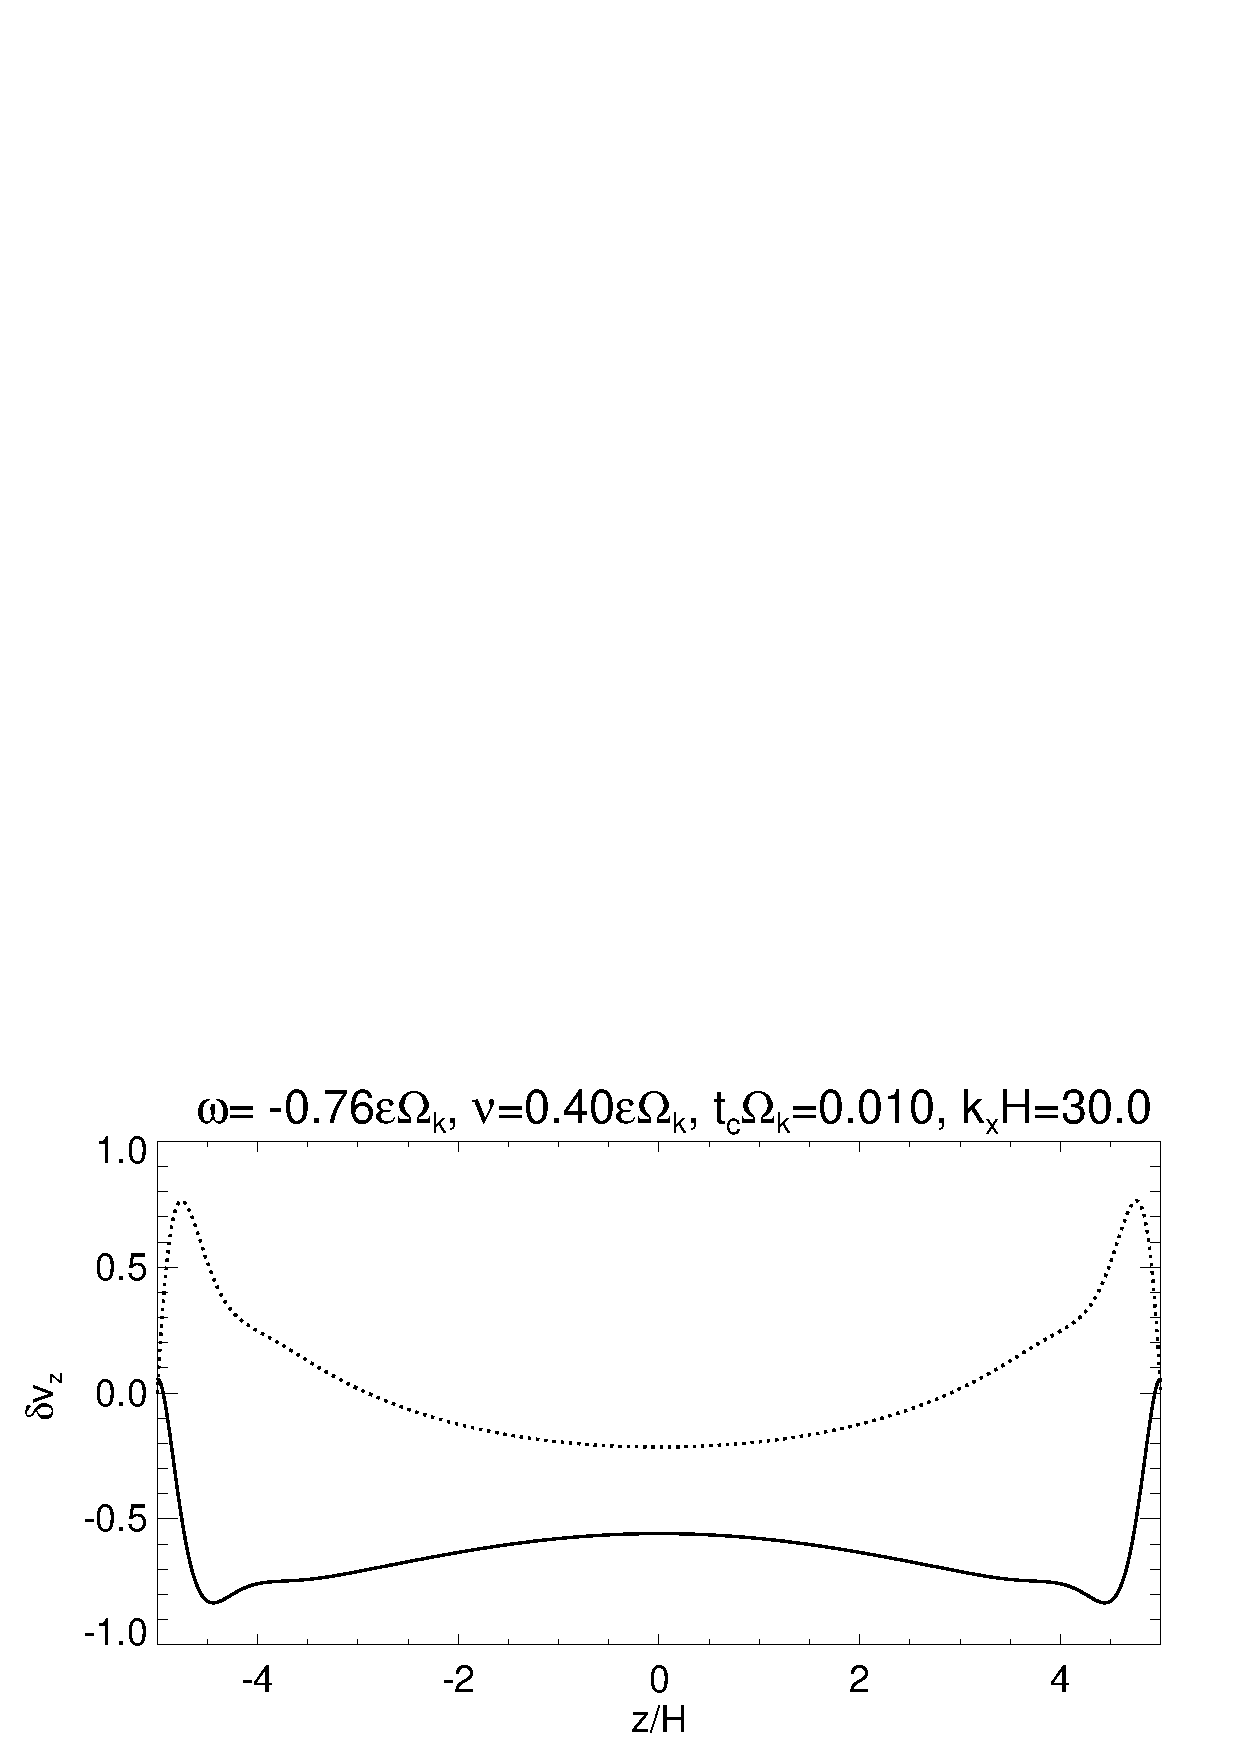
\includegraphics[width=\linewidth,clip=true,trim=0cm 1.75cm 0cm
  0cm]{figures/eigenvectorvz_beta0d01} 
  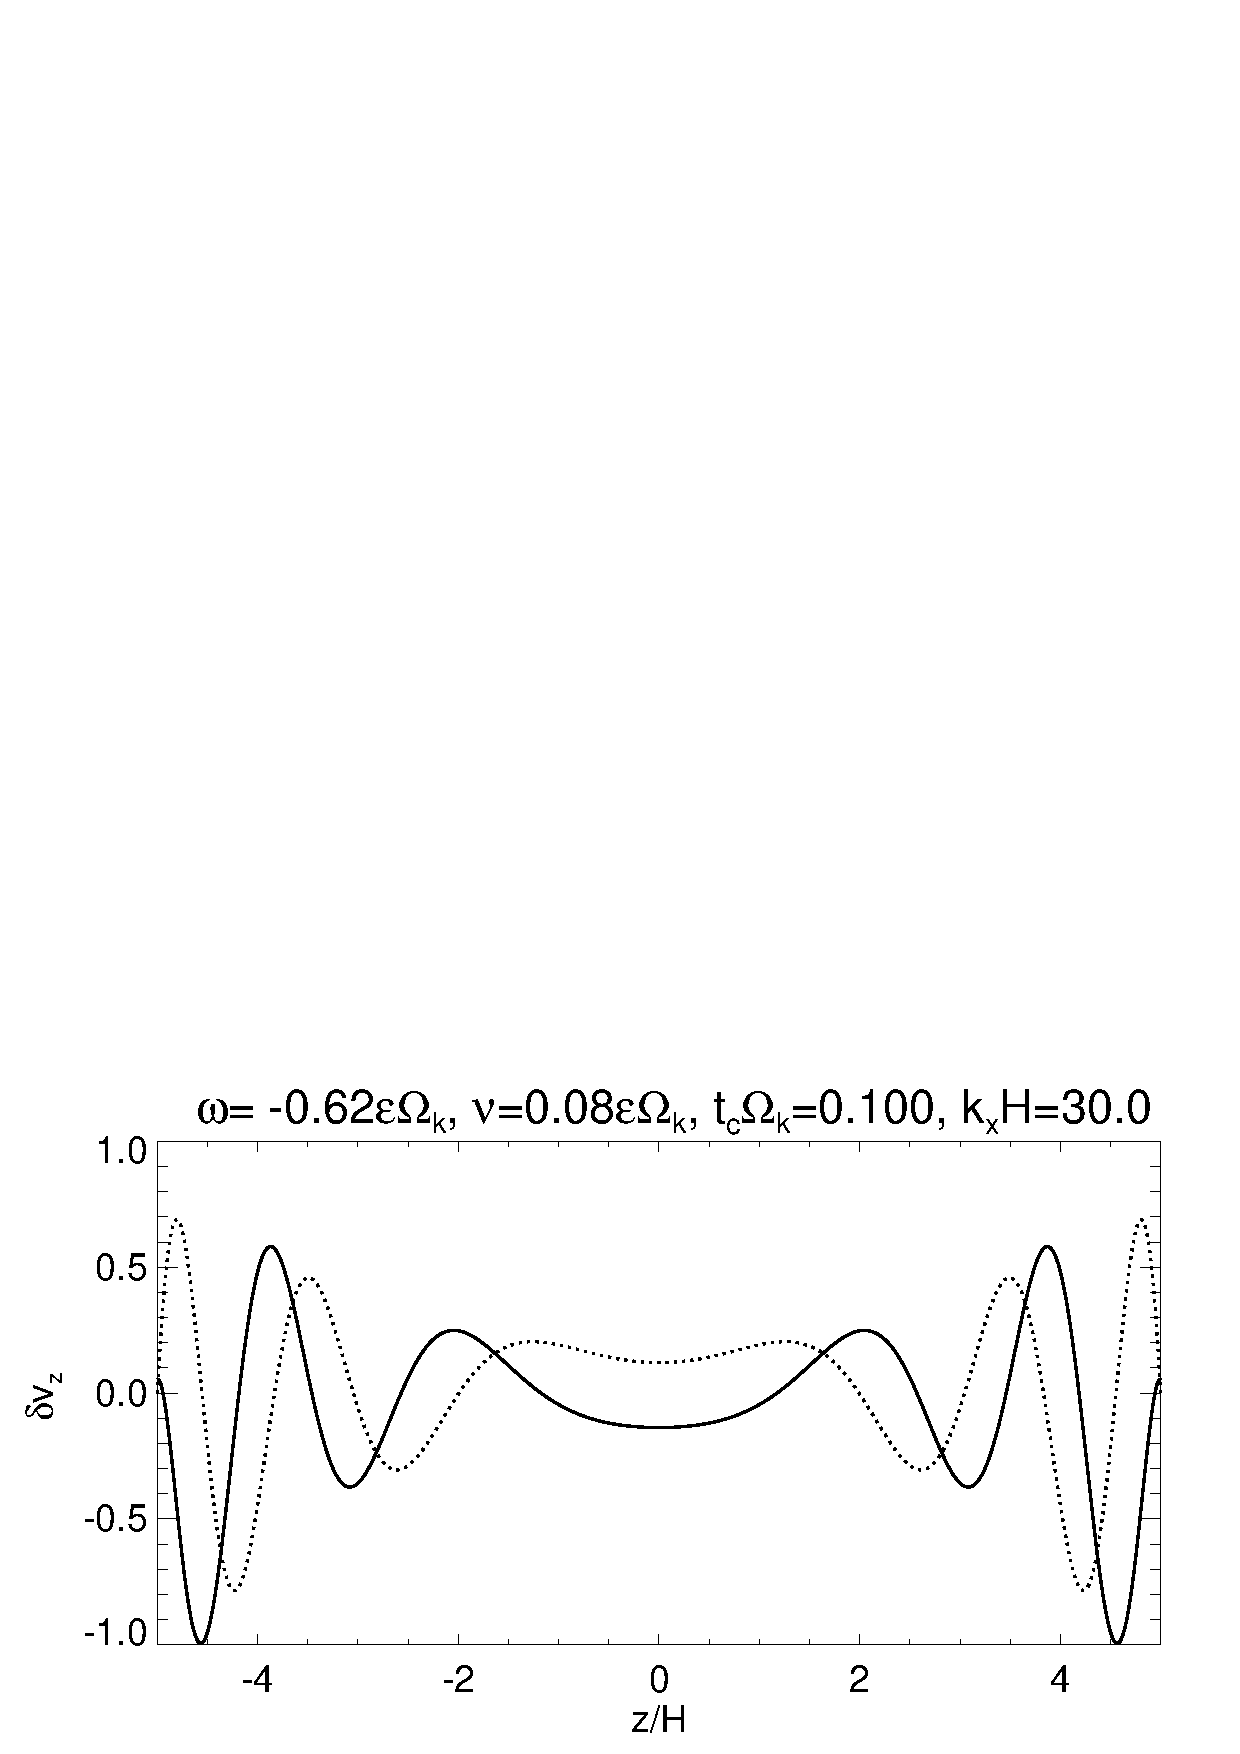
\includegraphics[width=\linewidth,clip=true,trim=0cm 0cm 0cm
  0cm]{figures/eigenvectorvz_beta0d1} 
  \caption{Numerically-calculated fundamental VSI
    mode in a nearly vertically isothermal disk ($\Gamma=1.011$) with
    $(p,q,\epsilon)=(-1.5,-1,0.05)$, evolved with $\gamma=1.4$ and a dimensionless 
    thermal relaxation timescale $\beta = 0.01$
    (top) and $\beta=0.1$ (bottom). The
    real (imaginary) part of the vertical velocity perturbation
    $\delta v_z$ is plotted as the solid (dotted)
    line. % The eigenfunction has been normalized such that
    % $\imag(\delta v_z)=0$ at the vertical boundaries, and
    % $\mathrm{max}|\delta v_z|=1$.
    \label{relax_eigenW_num}}  
\end{figure}

\subsection{Critical thermal relaxation timescale}\label{bcrit_num_test}
% may need to explain why choose k=10
% bcrit independent of k for k>>1 
% for some parameter regimes (e.g. large q, large epsilon) 
% behavior at larger kx and finite bcool not understood. 
We test the dependence of the critical thermal relaxation timescale 
$\beta_\mathrm{crit}$ for the fundamental VSI on disk parameters
(Eq. \ref{iso_vsi_cond}).  We use the previous case study as a
reference point and vary $q\in[-0.2,-1.2]$, 
$\gamma\in[1.2,2.0]$, and $\epsilon\in[0.02,0.1]$
separately. Here, we use a wavenumber $\khat=10$, for which we
find growth rates reach zero for the range of disk parameters
considered, so that a numerical $\beta_\mathrm{crit}$ can be defined precisely. 

The numerically-obtained $\beta_\mathrm{crit}$ is shown in
Fig. \ref{bcrit_compare} in comparison with Eq. \ref{iso_vsi_cond}.
Our numerical results generally agree with Eq. \ref{iso_vsi_cond}. The
agreement improves with decreasing  $|q|$,  $\epsilon$ and increasing
$\gamma$, i.e. weaker instability, although there is a noticeable difference
as $\gamma\to1$ because the derivation of $\beta_\mathrm{crit}$
assumed $\gamma>1$.   

Fig. \ref{bcrit_compare}, together with the previous section
(Fig. \ref{bcrit_compare1}), shows that $\beta_\mathrm{crit}$ as given
by Eq. \ref{iso_vsi_cond} gives a measure of the characteristic
thermal timescale below which perturbations are effectively isothermal
so that the fundamental VSI operates. 

% From the previous section (Fig. \ref{relax_eigenW_num}) we
% expect that for other wavenumbers,  still gives a characteristic
% thermal timescale below which the perturbations are effectively
% isothermal. 


\begin{figure}
  \includegraphics[width=\linewidth,clip=true,trim=0cm 0.cm 0cm
  0cm]{figures/bcrit_compare_q.ps} 
  \includegraphics[width=\linewidth,clip=true,trim=0cm 0.0cm 0cm
  0.8cm]{figures/bcrit_compare_g.ps}
  \includegraphics[width=\linewidth,clip=true,trim=0cm 0.0cm 0cm
  0.8cm]{figures/bcrit_compare_e.ps} 
  \caption{Dependence of the upper limit to the thermal relaxation timescale
    $\beta_\mathrm{crit}$ for the fundamental VSI mode on disk
    parameters. The fiducial parameters are $\Gamma=1.011$,
    $\gamma=1.4$ and $(p,q,\epsilon)=(-1.5,-1,0.05)$. Top: varying
    $q\in[-1.2,-0.2]$; middle: varying $\gamma\in[1.2,2.0]$; bottom:
    varying $\epsilon\in[0.02,0.1]$. The perturbation wavenumber is
    $\khat=10$.  
    \label{bcrit_compare}}  
\end{figure}

\subsection{Vertically non-isothermal disks} 
We briefly consider vertically non-isothermal disks with 
$\Gamma=1.4$ and $(p,q,\epsilon)=(0,-1,0.05)$ as simulated in
\cite{nelson13}. In this case we set $\zmax\simeq2.2H$, which
is close to the zero-density surface.      

Fig. \ref{gcorr_compare_vnoniso} plots the fundamental VSI growth
rates as a function of $\beta$ for $\gamma\in[1.4,2.5]$. In agreement with \citeauthor{nelson13}, in 
the neutrally-stratified case $\gamma=\Gamma$ the disk is unstable 
even for $\beta\gg 1$. (Note that in the adiabatic limit 
this disk can be unstable according to the
Solberg-Hoiland criterion, Eq. \ref{solberg2}.) 

For $\gamma>\Gamma$, i.e. stably stratified disks,
Fig. \ref{gcorr_compare_vnoniso} shows that introducing finite thermal
relaxation rapidly stabilizes the fundamental mode. This is
similar to that observed for nearly vertically isothermal disks
(Fig. \ref{bcrit_compare1}). For $\gamma=1.7,\,2.0,\,2.5$, growth
rates reach zero at  $\beta\simeq0.17,\,0.083,\,0.045$, respectively.
Interestingly, these values are equal to
$\epsilon|q|/(\gamma-\Gamma)$. This suggests that the critical thermal
relaxation timescale for vertically non-isothermal disks can also be
estimated by Eq. \ref{iso_vsi_cond} but with $\gamma-1$ replaced by
$\gamma-\Gamma$. 

\begin{figure}
  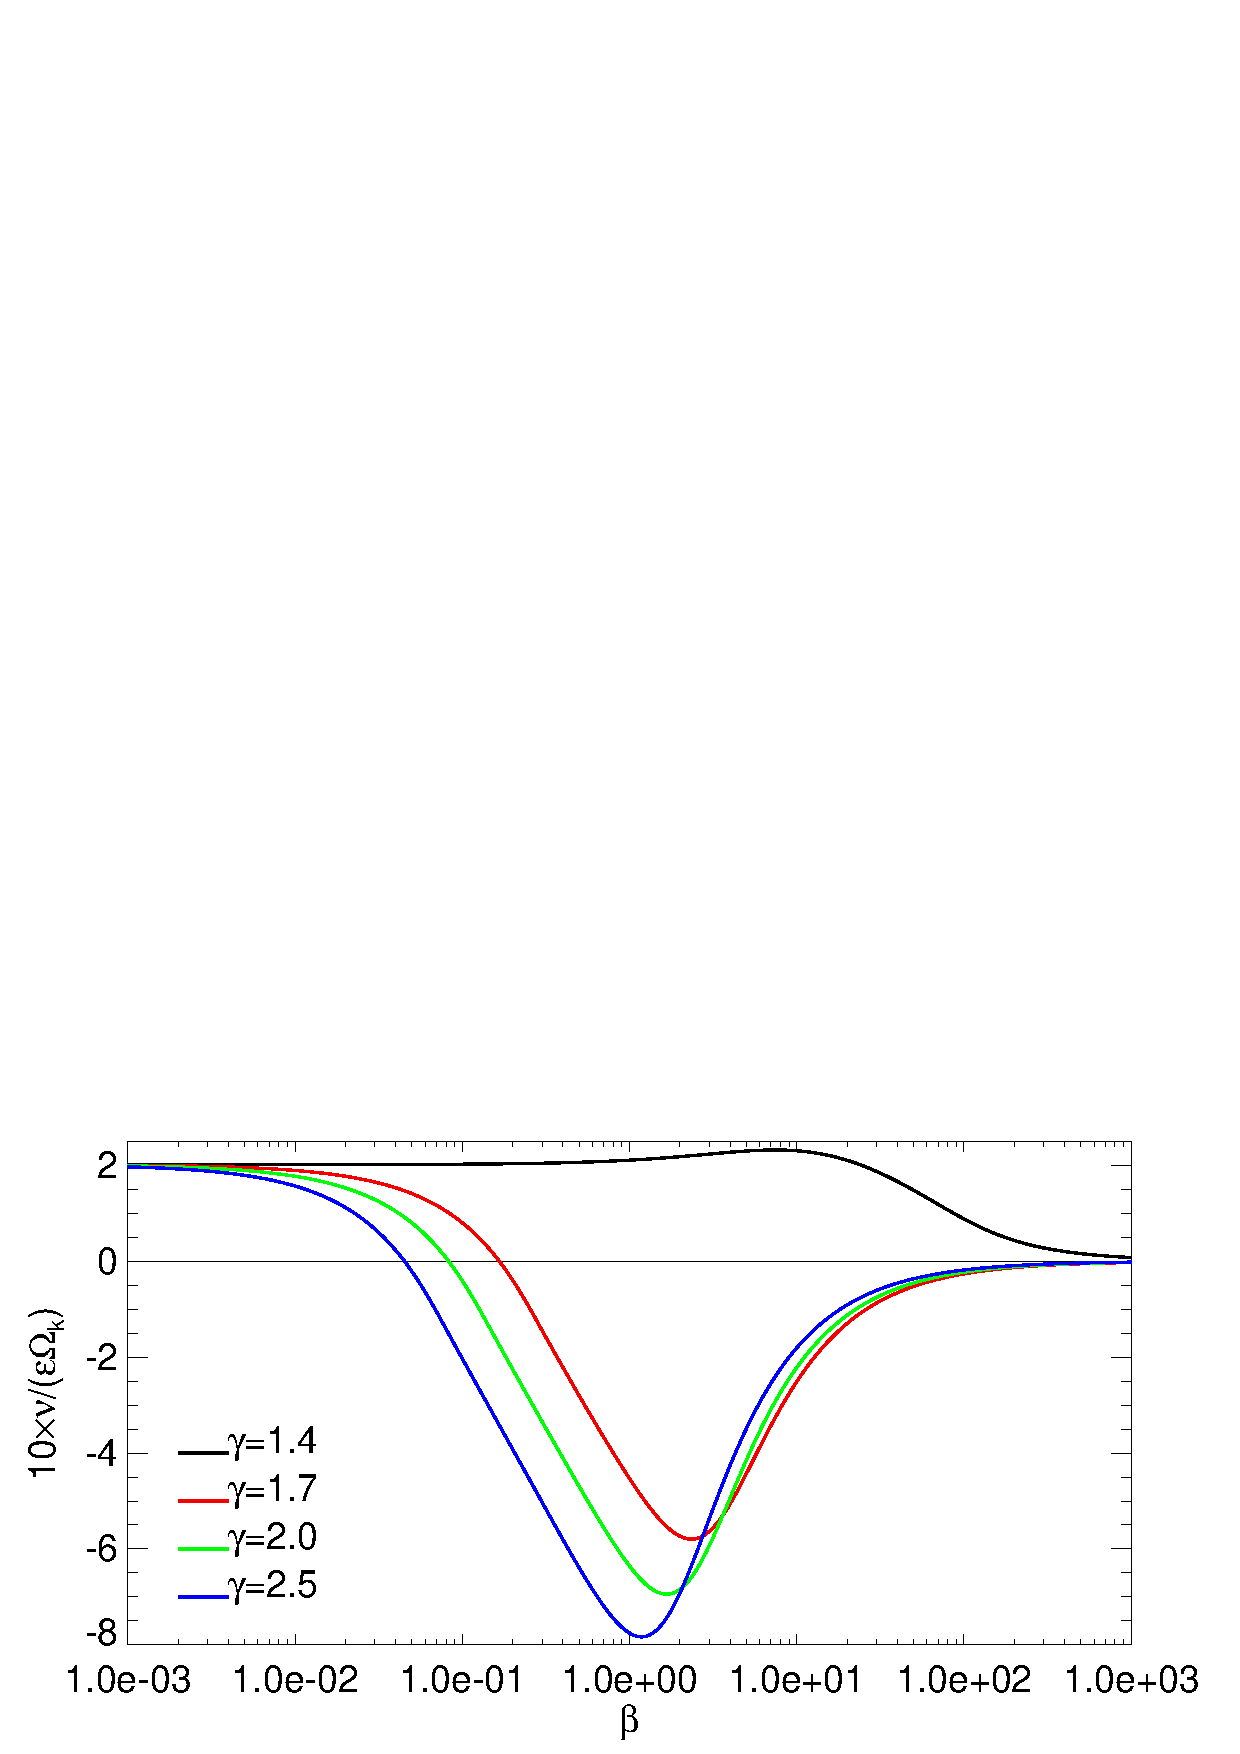
\includegraphics[width=\linewidth,clip=true,trim=0cm 0cm 0cm
  0cm]{figures/gcorr_compare_vnoniso2}
  \caption{Growth rate of the fundamental VSI mode as a function of
    the thermal relaxation timescale $\beta$, in vertically
    non-isothermal disks with $\Gamma=1.4$ and
    $\gamma\in[1.4,2.5]$. The disk is neutrally
    stratified for $\gamma=1.4$ and stably stratified for
    $\gamma>1.4$. Other disk parameters are
    $(p,q,\epsilon)=(0,-1,0.05)$ and the perturbation wavenumber is
    $\khat=30$.  
    \label{gcorr_compare_vnoniso}}
\end{figure}












% \subsection{VSI in a stably stratified disk}
% We demonstrate the (strong) stabilizing effect of a  
% positive vertical entropy gradient ($N_z^2\geq0$) by setting $\gamma=2$.  
% Since we expect the perturbations to decay rapidly
% away from the midplane (see \S\ref{analytic_adia}), we consider a
% smaller domain with $\zmax = 2\epsilon r$. 
% Other disk and perturbation parameters are the same as in
% \S\ref{vertiso_pertiso}.    

% Fig. \ref{lowfreq_eigen_adia} show the eigenvalues for this
% problem. The growth rates are much smaller than
% those in the previous section. The fundamental VSI mode is that with
% $\mathrm{max}\nu$. Its expected and numerically-calculated growth
% rates compares well, with 
% \begin{align*}
%   \nu = 0.03751 \epsilon \Omega_k &\quad \text{(from
%     Eq. \ref{gam2_growth_rate})},\\
%   \nu = 0.03672 \epsilon \Omega_k &\quad \text{(numerical)}.
% \end{align*}
% The fundamental mode is plotted in Fig. \ref{lowfreq_eigenfunc_adia},
% and clearly show that perturbations are rapidly stabilized away from
% the midplane. For the adopted disk and perturbation parameters,
% Eq. \ref{gam2_alpha} gives $\real{\alpha}\simeq - 43.8$, corresponding
% to a characteristic decay length scale of $\sqrt{2/|\alpha|}\epsilon r\simeq 0.2\epsilon r$,
% which is consistent with that observed in  Fig. \ref{lowfreq_eigenfunc_adia}. 

% This decay lengthscale is rougly the height within which
% vertical shear is larger than the buoyancy frequency squared. That is,
% \begin{align*}
% \left|r\frac{d\Omega^2}{dz}\right|\gtrsim N_z^2
% \end{align*}
% for
% \begin{align*}
%   \left|\frac{z}{\epsilon r}\right| \lesssim \frac{\epsilon|q|\gamma}{\gamma-1},
% \end{align*}
% in a thin, vertically isothermal disk. This evaluates to $|z|\lesssim
% 0.2\epsilon r$ for the current disk model, consistent with
% Fig. \ref{lowfreq_eigenfunc_adia}. 

% Furthermore, the growth rate to should be no larger than the
% maximum vertical shear available within this decay lengthscale. Using 
% Eq. \ref{max_growth} as a rough guide, 
% \begin{align}
%   \frac{\nu}{\epsilon\Omega_k}<\frac{\epsilon |q|^2\gamma}{2(\gamma-1)},
% \end{align}
% or $\nu< 0.1\epsilon\Omega_k$ in our disk model,
% consistent with numerical results. 

% \begin{figure}
%   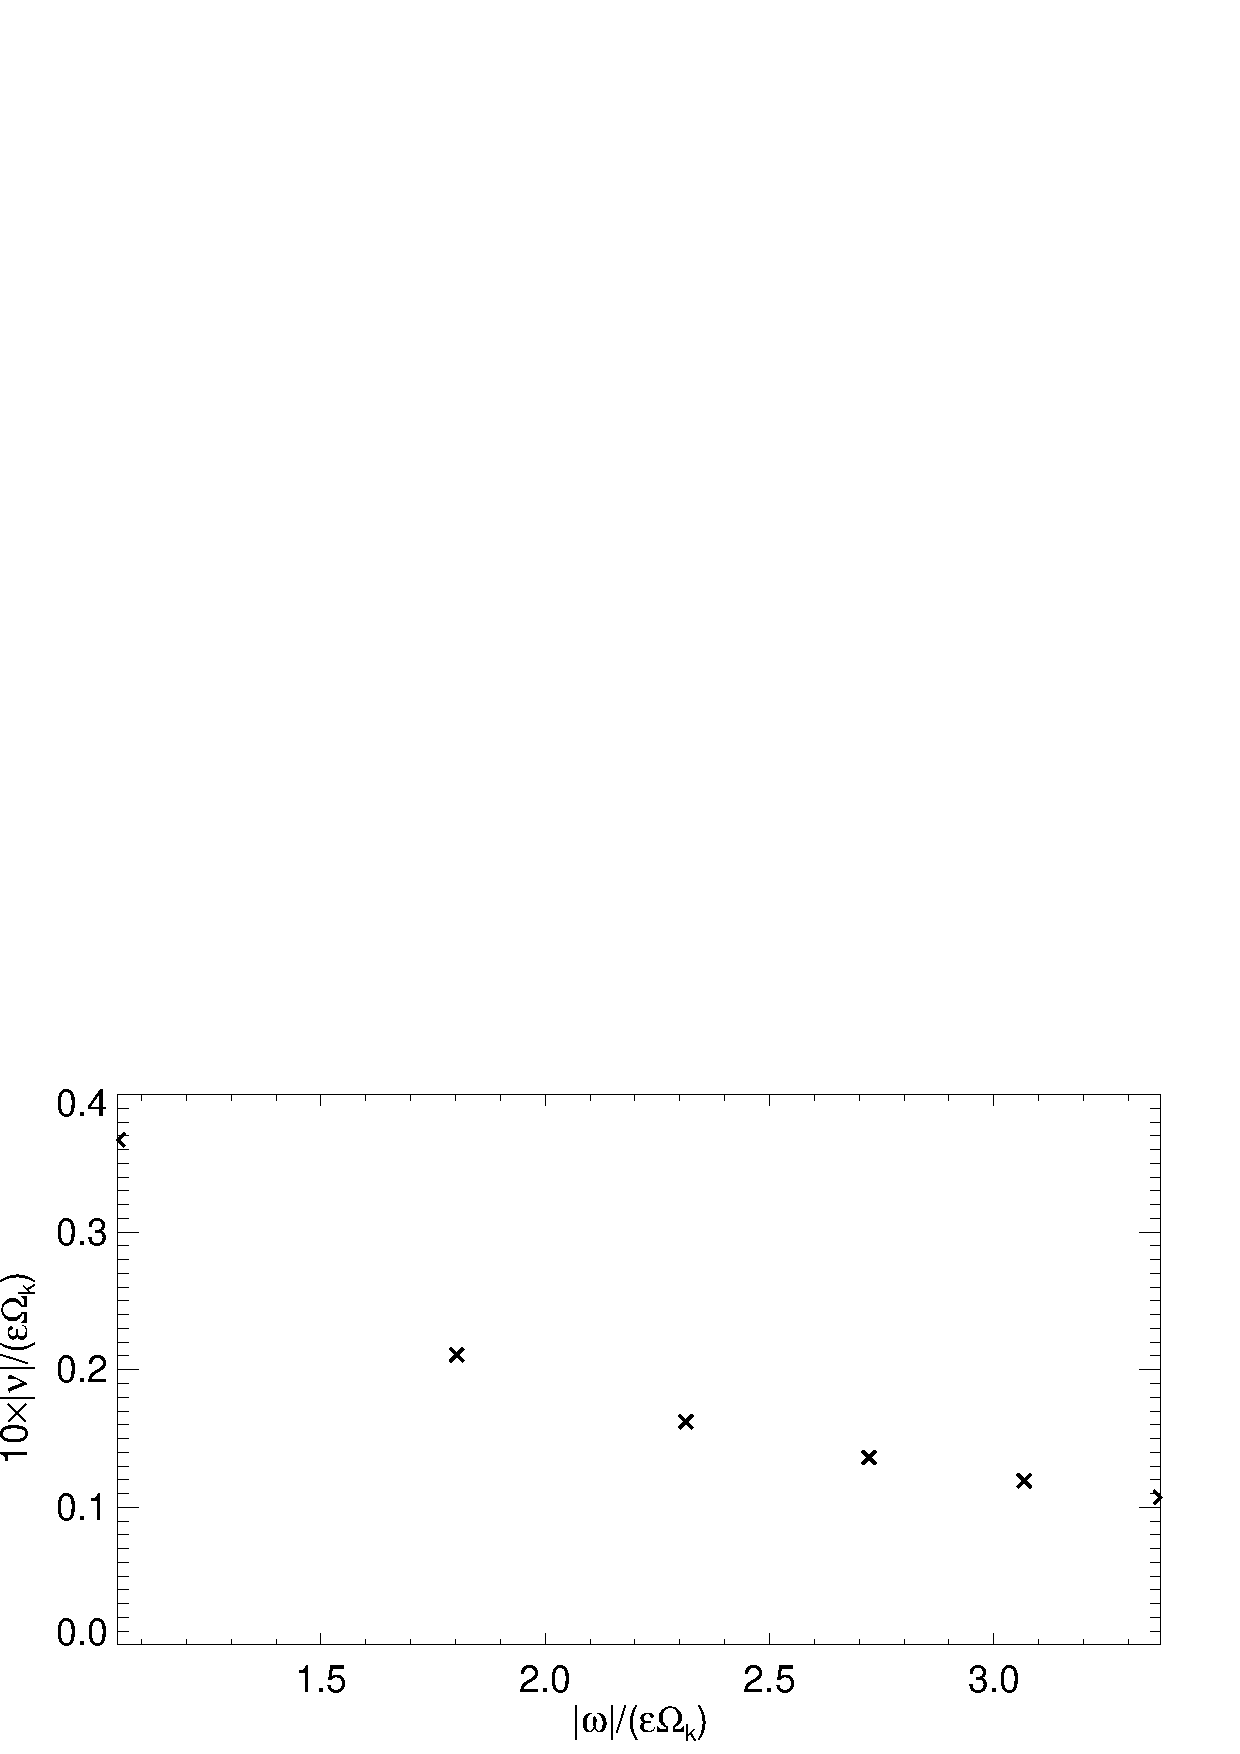
\includegraphics[width=\linewidth]{figures/eigenvalues_adia}
%   \caption{Eigenvalues in for the
%     VSI in a nearly vertically isothermal disk
%     ($\Gamma=1.011$) with $(p,q,\epsilon)=(-1.5,-1,0.1)$, 
%     evolved adiabatically with $\gamma=2$. The perturbation radial
%     wavenumber is $\khat=20\pi$. \label{lowfreq_eigen_adia}
%   }
% \end{figure}
  

% \begin{figure}
%   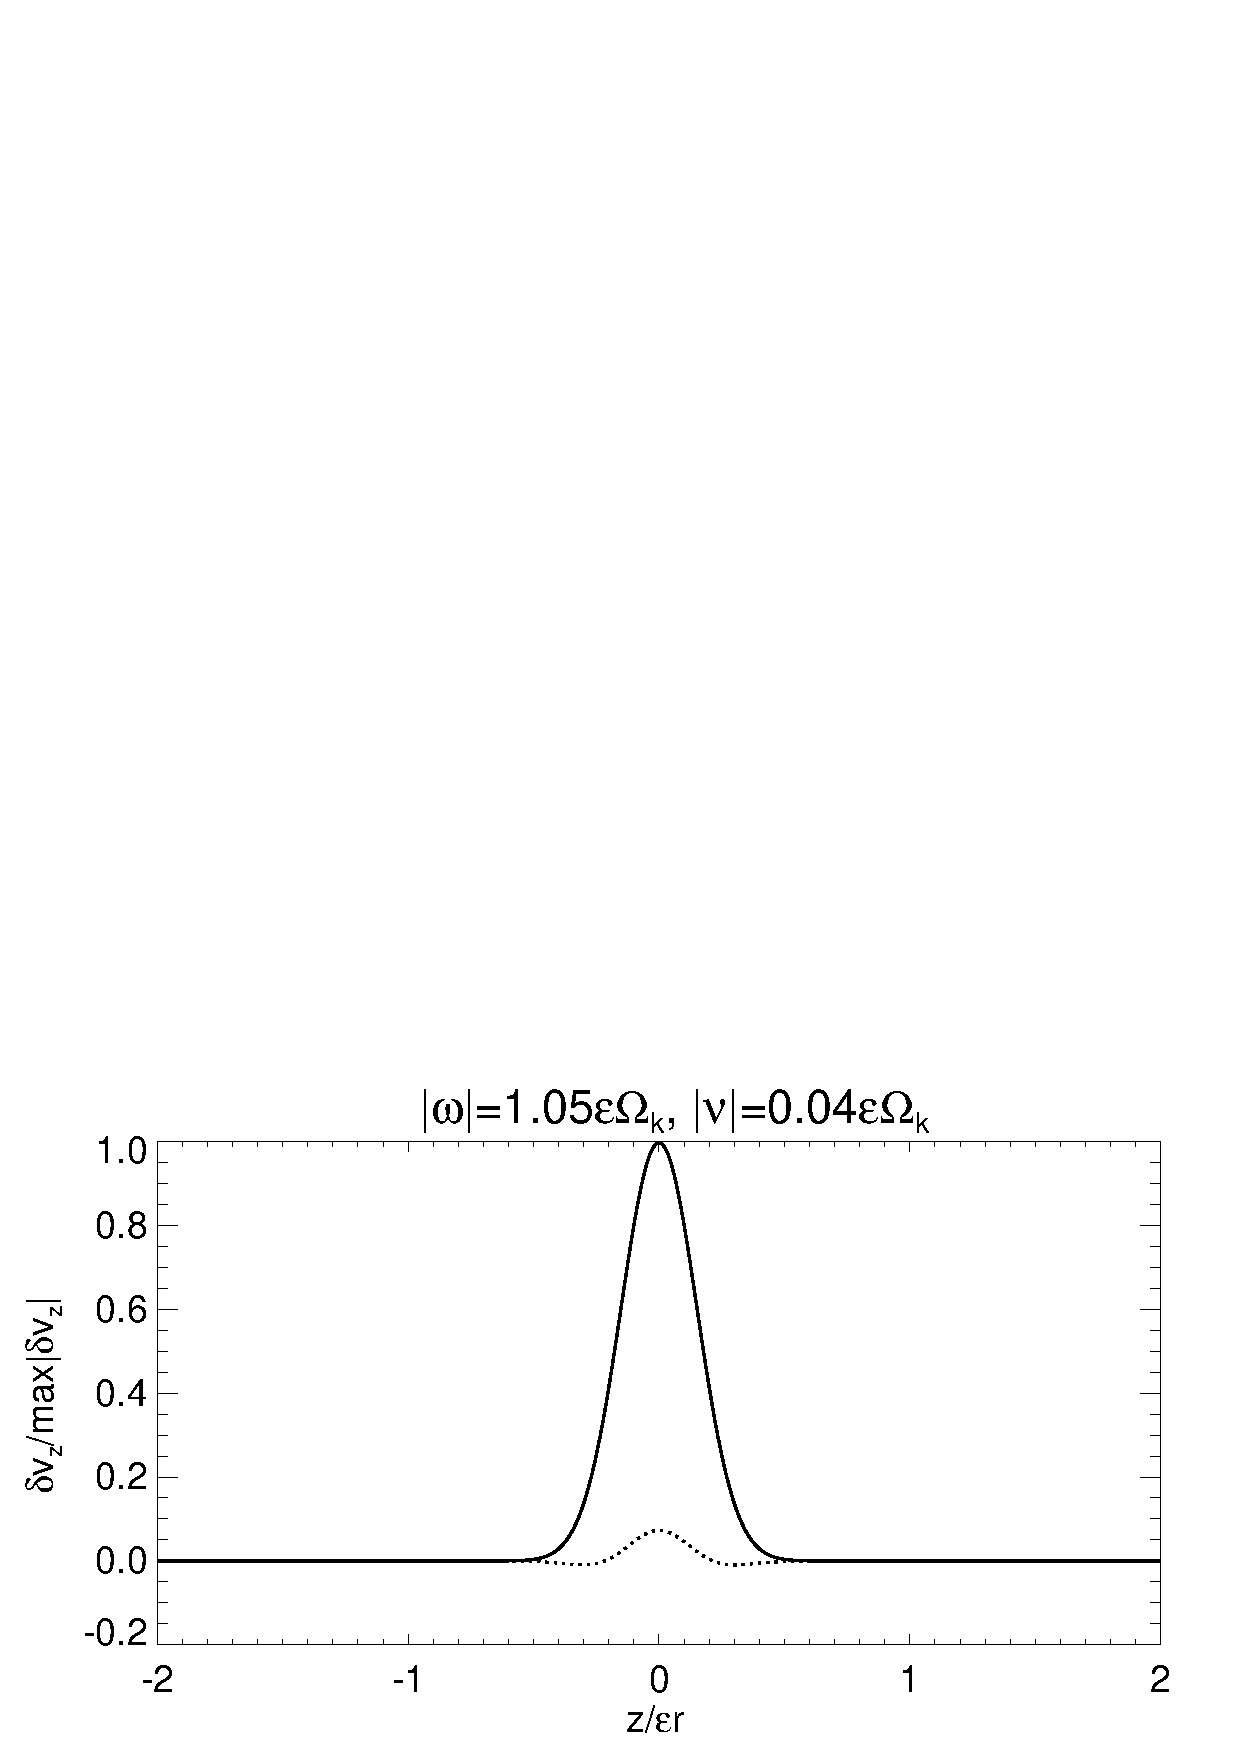
\includegraphics[width=\linewidth]{figures/eigenvectorvz_adia}
%   \caption{Fundamental VSI mode in a nearly vertically
%     isothermal disk ($\Gamma=1.011$) with $(p,q,\epsilon)=(-1.5,-1,0.1)$, 
%     evolved adiabatically
%     with $\gamma=2$. This eigenfunction 
%     corresponds to the top-left eigenvalue displayed in 
%     Fig. \ref{lowfreq_eigen_adia} (largest $|\nu|$).  
%     The  real (imaginary) part of $\delta v_z$ are shown as solid
%     (dotted) lines. 
%     \label{lowfreq_eigenfunc_adia}
%   }
% \end{figure}

% Although a positive vertical entropy gradient is stabilizing, we note
% that $N_z^2\propto z^2$  while vertical shear $rd\Omega^2/dz\propto
% z$, so that there is always a region sufficiently close to the
% midplane in which vertical shear dominates over bouyancy and the VSI
% can operate. However, the growth rates are small and the instability
% only affects the regions close the midplane. These modes may not be
% important in practice.  


% \subsection{Other adiabatic indices}
% To see the transition from neutrally-bouyant to stably stratified cases above, 
% we repeated the previous calculation with $\gamma\in[1,2]$. 
% We restore the vertical domain to $\zmax=10\epsilon r$. 
% Fig. \ref{adia_growth_num} shows the eigenfrequencies of the
% fundamental VSI mode. 


% %To select the appropriate
% %eigenvalues we vary the parameters slowly away from a reference solution.   
% % The numerically-determined eigenfrequencies are qualitatively
% % consistent with the discussion in \S\ref{adia_compare_gam1}.
% There is good agreement between Fig. \ref{adia_growth_num} and
% Fig. \ref{adia_growth} for $\khat=k_xH\gtrsim1$. There is a
% mismatch for smaller wavenumbers, especially in the growth
% rates. Actual growth rates decrease slower as $\khat\to0$
% than that in Fig. \ref{adia_growth}. Disagreement at small
% $\khat$ is not unexpected because the low-frequency
% approximation used to obtain Fig. \ref{adia_growth} becomes invalid since
% $|\omega|\sim\Omega_k$ for small $\khat$.  

% Given the number of approximations made in \S\ref{adia_compare_gam1},
% Fig. \ref{adia_growth_num} compares well with 
% Fig. \ref{adia_growth}. The main qualitative features of the full
% numerical solution in Fig. \ref{adia_growth_num} are captured by
% Fig. \ref{adia_growth}: stabilization for 
% $\khat\to0$ and $\khat\to\infty$,
% stabilization for increasing $\gamma$ (but ineffective at small $\khat$), 
% and the shift of the most unstable wavenumber to smaller values as
% $\gamma$ is increased. 


% \begin{figure}
%   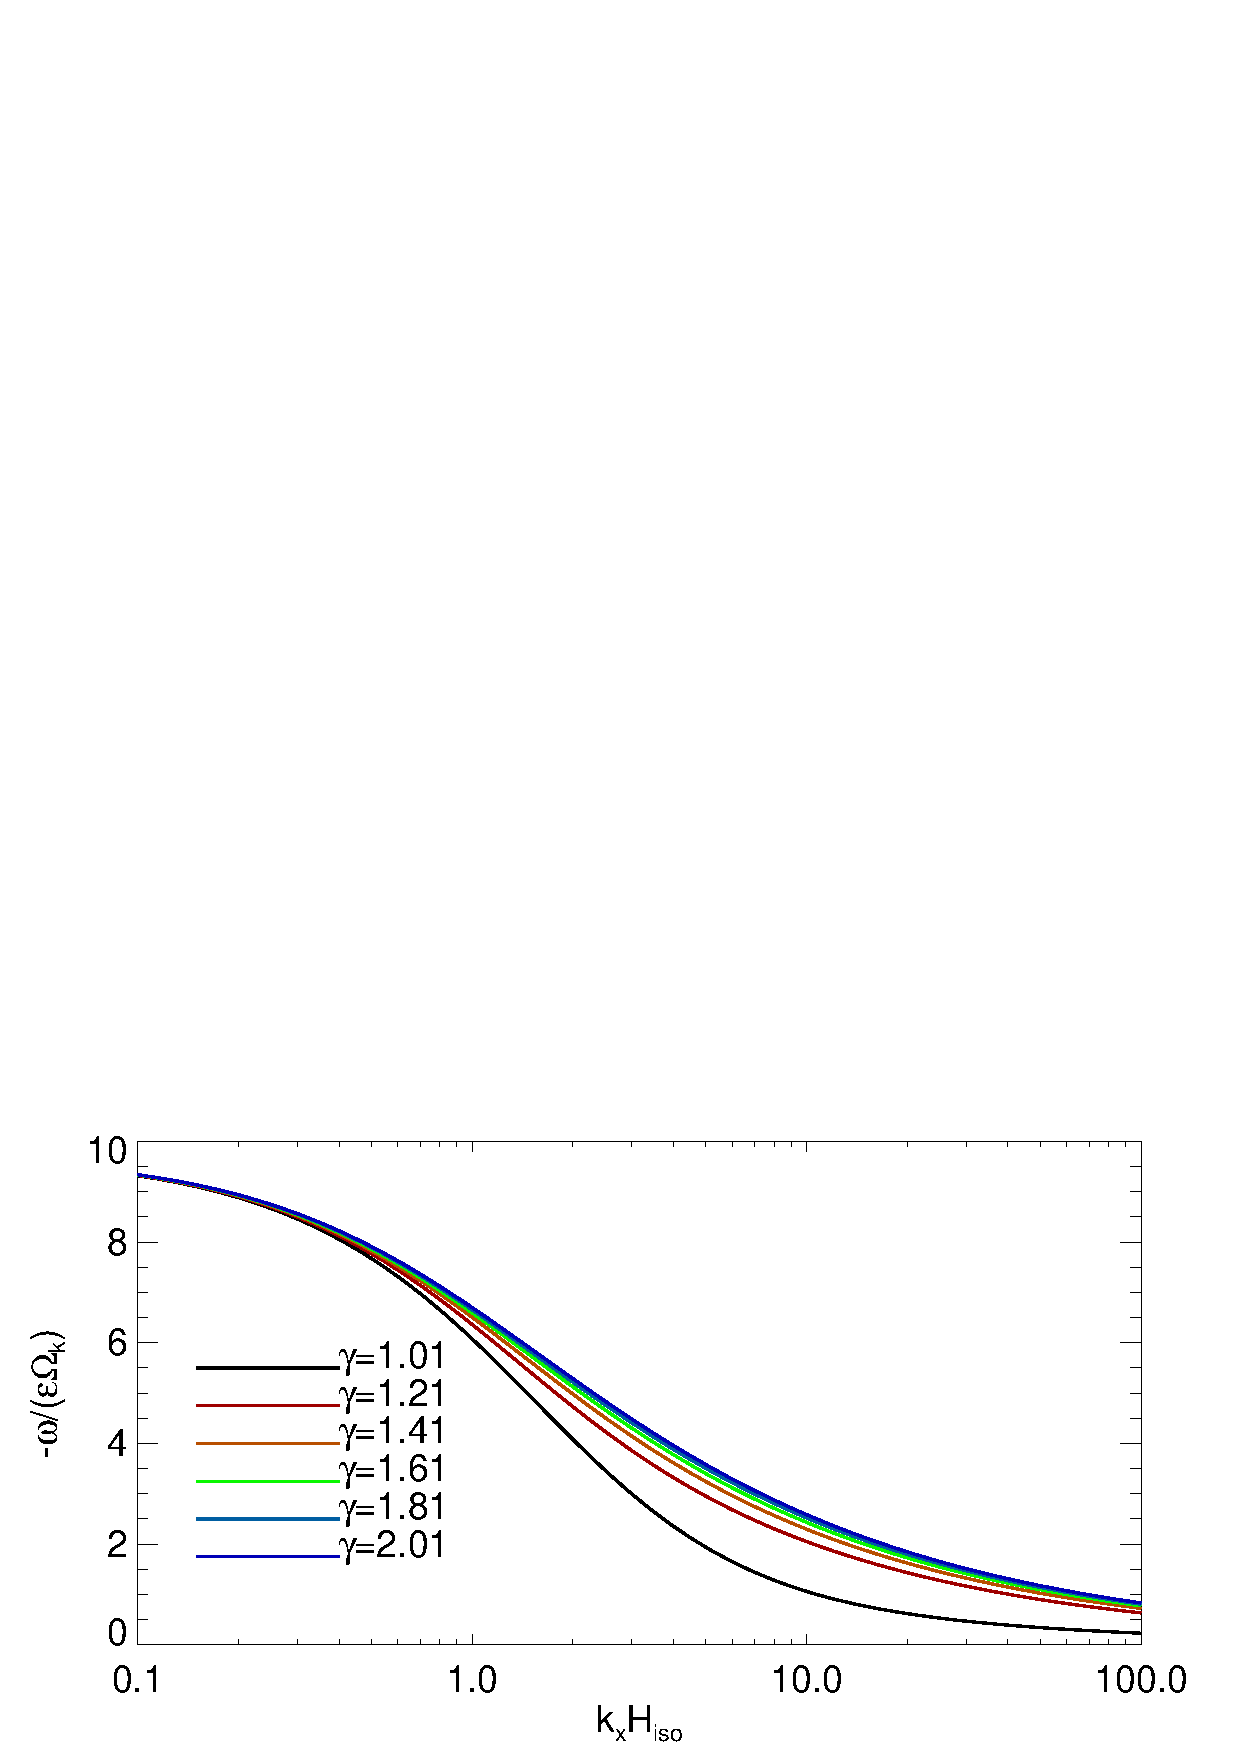
\includegraphics[width=\linewidth,clip=true,trim=0cm 1.75cm 0cm 0cm]{figures/compare_eigen_real1}
%   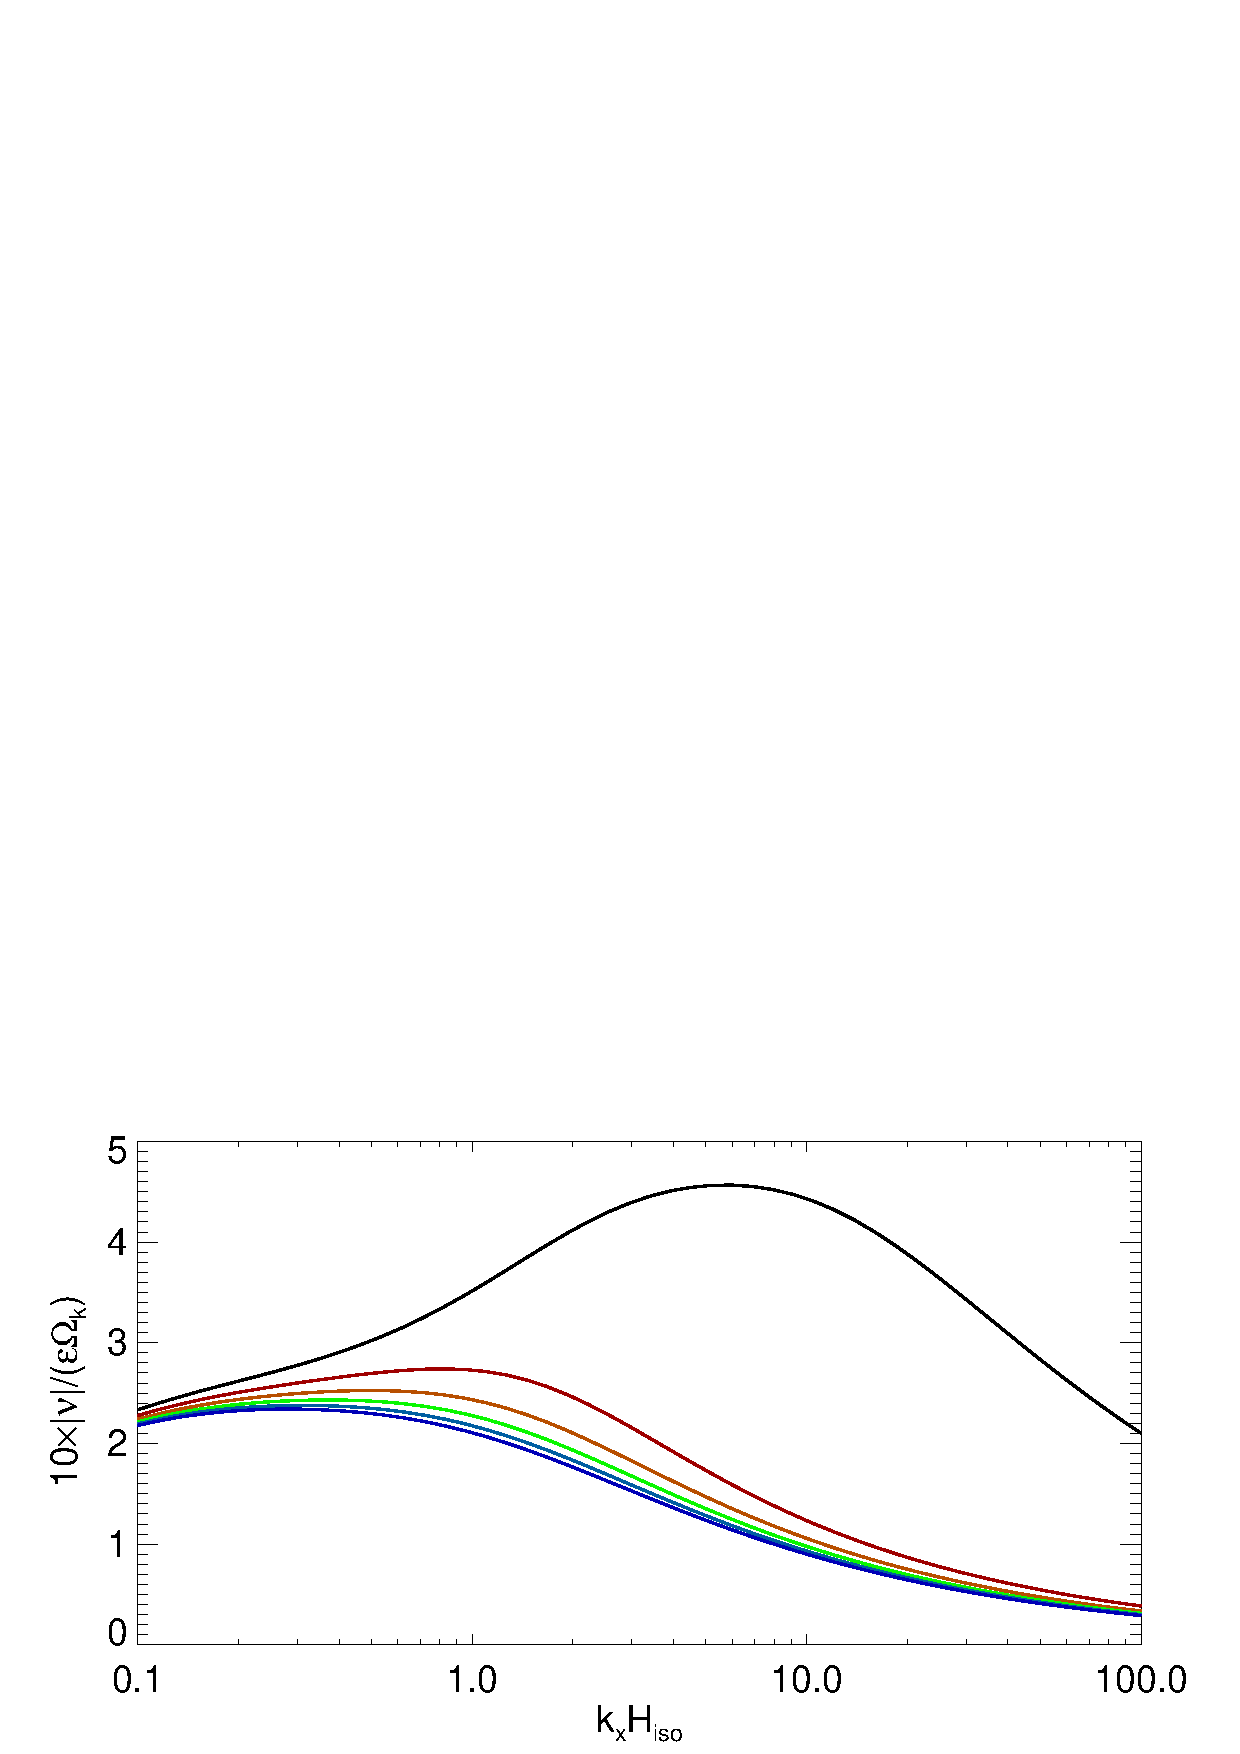
\includegraphics[width=\linewidth,clip=true,trim=0cm 0cm 0cm 1cm]{figures/compare_eigen_imag1}
%   \caption{Real frequency (top) and growth rate 
%     (bottom) of the fundamental VSI in a nearly vertically   
%     isothermal disks ($\Gamma=1.011$) with $(p,q,\epsilon)=(-1.5,-1,0.1)$, 
%     subject to adiabatic perturbations with different values of $\gamma$. 
%     The eigenfrequencies are calculated by numerically
%     solving the full linear eigenvalue problem. This plot is to
%     be compared with Fig. \ref{adia_growth}. \label{adia_growth_num}}   
% \end{figure}  
